%% 使用 njuthesis 文档类生成南京大学学位论文的示例文档
%%
%% 作者:胡海星,starfish (at) gmail (dot) com
%% 项目主页: http://haixing-hu.github.io/nju-thesis/
%%
%% 本样例文档中用到了吕琦同学的博士论文的提高和部分内容,在此对他表示感谢。
%%
\documentclass[macfonts,master]{njuthesis}
%% njuthesis 文档类的可选参数有:
%%   nobackinfo 取消封二页导师签名信息。注意,按照南大的规定,是需要签名页的。
%%   phd/master/bachelor 选择博士/硕士/学士论文

% 使用 blindtext 宏包自动生成章节文字
% 这仅仅是用于生成样例文档,正式论文中一般用不到该宏包
%\usepackage[math]{blindtext}
\usepackage{listings}
\usepackage{xcolor}

\newcommand\YAMLcolonstyle{\color{red}\mdseries}
\newcommand\YAMLkeystyle{\color{black}\bfseries}
\newcommand\YAMLvaluestyle{\color{blue}\mdseries}

\makeatletter

% here is a macro expanding to the name of the language
% (handy if you decide to change it further down the road)
\newcommand\language@yaml{yaml}

\expandafter\expandafter\expandafter\lstdefinelanguage
\expandafter{\language@yaml}
{
  keywords={true,false,null,y,n},
  keywordstyle=\color{darkgray}\bfseries\small,
  basicstyle=\YAMLkeystyle\small,                                 % assuming a key comes first
  numbers=left,
  numberstyle=\footnotesize,
  frame=single,
  breaklines,
  columns=flexible,
  sensitive=false,
  comment=[l]{\#},
  morecomment=[s]{/*}{*/},
  commentstyle=\color{purple}\ttfamily,
  stringstyle=\YAMLvaluestyle\ttfamily\small,
  moredelim=[l][\color{orange}]{\&},
  moredelim=[l][\color{magenta}]{*},
  moredelim=**[il][\YAMLcolonstyle{:}\YAMLvaluestyle]{:},   % switch to value style at :
  morestring=[b]',
  morestring=[b]",
  literate =    {---}{{\ProcessThreeDashes}}3
                {>}{{\textcolor{red}\textgreater}}1
                {|}{{\textcolor{red}\textbar}}1
                {\ -\ }{{\mdseries\ -\ }}3,
}

% switch to key style at EOL
\lst@AddToHook{EveryLine}{\ifx\lst@language\language@yaml\YAMLkeystyle\fi}
\makeatother

\newcommand\ProcessThreeDashes{\llap{\color{cyan}\mdseries-{-}-}}

%\usepackage[utf8]{inputenc}
%\usepackage[english]{babel}
%
%\usepackage[outputdir=.texpadtmp]{minted}
%\usemintedstyle{borland}

\usepackage{color}
\usepackage{xcolor}

\definecolor{lightgray}{rgb}{.9,.9,.9}
\definecolor{darkgray}{rgb}{.4,.4,.4}
\definecolor{purple}{rgb}{0.65, 0.12, 0.82}

\lstdefinelanguage{Go}{
  % Keywords as defined in the language grammar
  morekeywords=[1]{%
    break,default,func,interface,select,case,defer,go,map,%
    struct,chan,else,goto,package,switch,const,fallthrough,%
    if,range,type, continue,for,import,return,var},
  % Built-in functions
  morekeywords=[2]{%
    append,cap,close,complex,copy,delete,imag,%
    len,make,new,panic,print,println,real,recover},
  % Pre-declared types
  morekeywords=[3]{%
    bool,byte,complex64,complex128,error,float32,float64,%
    int,int8,int16,int32,int64,rune,string,%
    uint,uint8,uint16,uint32,uint64,uintptr},
  % Constants and zero value
  morekeywords=[4]{true,false,iota,nil},
  % Strings : "foo", 'bar', `baz`
  morestring=[b]{"},
  morestring=[b]{'},
  morestring=[b]{`},
  % Comments : /* comment */ and // comment
  comment=[l]{//},
  morecomment=[s]{/*}{*/},
  basicstyle=\ttfamily\small,
  numbers=left,
  numberstyle=\footnotesize,
  frame=single,
  breaklines,
  columns=flexible,
  keywordstyle=\color{blue}\ttfamily,
  stringstyle=\color{red}\ttfamily,
  commentstyle=\color{green}\ttfamily,
  tabsize=4,
  % Options
  sensitive=true
}

\lstdefinelanguage{JavaScript}{
  basicstyle=\ttfamily\small,
  numbers=left,
  numberstyle=\footnotesize,
  frame=single,
  breaklines,
  columns=flexible,
  keywords={typeof, new, true, false, catch, function, return, null, catch, switch, var, if, in, while, do, else, case, break},
  keywordstyle=\color{blue}\bfseries,
  ndkeywords={class, export, boolean, throw, implements, import, this},
  ndkeywordstyle=\color{darkgray}\bfseries,
  identifierstyle=\color{black},
  sensitive=false,
  comment=[l]{//},
  morecomment=[s]{/*}{*/},
  commentstyle=\color{purple}\ttfamily,
  stringstyle=\color{red}\ttfamily,
  morestring=[b]',
  morestring=[b]"
}

\colorlet{punct}{red!60!black}
\definecolor{background}{HTML}{EEEEEE}
\definecolor{delim}{RGB}{20,105,176}
\colorlet{numb}{magenta!60!black}

\lstdefinelanguage{json}{
    basicstyle=\ttfamily\small,
    numbers=left,
    numberstyle=\footnotesize,
    frame=single,
  	breaklines,
  	columns=flexible,
    stepnumber=1,
    numbersep=8pt,
    showstringspaces=false,
    breaklines=true,
    frame=lines,
    backgroundcolor=\color{background},
    literate=
     *{0}{{{\color{numb}0}}}{1}
      {1}{{{\color{numb}1}}}{1}
      {2}{{{\color{numb}2}}}{1}
      {3}{{{\color{numb}3}}}{1}
      {4}{{{\color{numb}4}}}{1}
      {5}{{{\color{numb}5}}}{1}
      {6}{{{\color{numb}6}}}{1}
      {7}{{{\color{numb}7}}}{1}
      {8}{{{\color{numb}8}}}{1}
      {9}{{{\color{numb}9}}}{1}
      {:}{{{\color{punct}{:}}}}{1}
      {,}{{{\color{punct}{,}}}}{1}
      {\{}{{{\color{delim}{\{}}}}{1}
      {\}}{{{\color{delim}{\}}}}}{1}
      {[}{{{\color{delim}{[}}}}{1}
      {]}{{{\color{delim}{]}}}}{1},
}

%%%%%%%%%%%%%%%%%%%%%%%%%%%%%%%%%%%%%%%%%%%%%%%%%%%%%%%%%%%%%%%%%%%%%%%%%%%%%%%
% 设置《国家图书馆封面》的内容,仅博士论文才需要填写

% 设置论文按照《中国图书资料分类法》的分类编号
\classification{0175.2}
% 论文的密级。需按照GB/T 7156-2003标准进行设置。预定义的值包括:
% - \openlevel,表示公开级:此级别的文献可在国内外发行和交换。
% - \controllevel,表示限制级:此级别的文献内容不涉及国家秘密,但在一定时间内
%   限制其交流和使用范围。
% - \confidentiallevel,表示秘密级:此级别的文献内容涉及一般国家秘密。
% - \clasifiedlevel,表示机密级:此级别的文献内容涉及重要的国家秘密 。
% - \mostconfidentiallevel,表示绝密级:此级别的文献内容涉及最重要的国家秘密。
% 此属性可选,默认为\openlevel,即公开级。
\securitylevel{\controllevel}
% 设置论文按照《国际十进分类法UDC》的分类编号
% 该编号可在下述网址查询:http://www.udcc.org/udcsummary/php/index.php?lang=chi
\udc{004.72}
% 国家图书馆封面上的论文标题第一行,不可换行。此属性可选,默认值为通过\title设置的标题。
\nlctitlea{声明式的通用Kubernetes}
% 国家图书馆封面上的论文标题第二行,不可换行。此属性可选,默认值为空白。
\nlctitleb{Operator的设计与实现}
% 国家图书馆封面上的论文标题第三行,不可换行。此属性可选,默认值为空白。
\nlctitlec{}
% 导师的单位名称及地址
\supervisorinfo{南京大学计算机科学与技术系~~南京市栖霞区仙林大道163号~~210023}
% 答辩委员会主席
\chairman{~~教授}
% 第一位评阅人
\reviewera{~~教授}
% 第二位评阅人
\reviewerb{~~副教授}
% 第三位评阅人
\reviewerc{~~教授}
% 第四位评阅人
\reviewerd{~~研究员}

%%%%%%%%%%%%%%%%%%%%%%%%%%%%%%%%%%%%%%%%%%%%%%%%%%%%%%%%%%%%%%%%%%%%%%%%%%%%%%%
% 设置论文的中文封面

% 论文标题,不可换行
\title{声明式的通用Kubernetes Operator的设计与实现}
\titlea{声明式的通用Kubernetes}
\titleb{Operator的设计与实现}
% 如果论文标题过长,可以分两行,第一行用\titlea{}定义,第二行用\titleb{}定义,将上面的\title{}注释掉
% \titlea{半轻衰变$D^+\to \omega(\phi)e^+\nu_e$的研究}
% \titleb{和弱衰变$J/\psi \to D_s^{(*)-}e^+\nu_e$的寻找}

%%盲审命令,空白字段设置请看.cls文件\newcommand*{\blind}
%此外,请按照盲审要求自行去掉个人简历、致谢等页面中的个人信息
\blind

% 论文作者姓名
%\author{汪浩港}
%% 论文作者联系电话
%\telphone{15605213809}
%% 论文作者电子邮件地址
%\email{whg19961229@gmail.com}
%% 论文作者学生证号
%\studentnum{MG1833067}
%% 论文作者入学年份(年级)
%\grade{2018}
%% 导师姓名职称
%\supervisor{曹春~~教授}
%% 导师的联系电话
%\supervisortelphone{18951679203}
%% 论文作者的学科与专业方向
%\major{计算机科学与技术}
%% 论文作者的研究方向
%\researchfield{软件方法学}

% 论文作者所在院系的中文名称
\department{计算机科学与技术系}
% 论文作者所在学校或机构的名称。此属性可选,默认值为``南京大学''。
\institute{南京大学}
% 论文的提交日期,需设置年、月、日。
\submitdate{2021年4月15日}
% 论文的答辩日期,需设置年、月、日。
\defenddate{2021年6月1日}
% 论文的定稿日期,需设置年、月、日。此属性可选,默认值为最后一次编译时的日期,精确到日。
%% \date{2013年5月1日}
% 论文的定稿日期,需设置年、月、日。此属性可选,默认值为最后一次编译时的日期,精确到日。
%% \date{2013年5月1日}

%%%%%%%%%%%%%%%%%%%%%%%%%%%%%%%%%%%%%%%%%%%%%%%%%%%%%%%%%%%%%%%%%%%%%%%%%%%%%%%
% 设置论文的英文封面

% 论文的英文标题,不可换行
\englishtitle{The Design and Implementation of A Kubernetes Operator Which is Declarative and Universal}
% 论文作者姓名的拼音
%\englishauthor{Wang Haogang}
%% 导师姓名职称的英文
%\englishsupervisor{Professor Cao Chun}
%% 论文作者学科与专业的英文名
%\englishmajor{Computer Science and Technology}
% 论文作者所在院系的英文名称
\englishdepartment{Department of Computer Science and Technology}
% 论文作者所在学校或机构的英文名称。此属性可选,默认值为``Nanjing University''。
\englishinstitute{Nanjing University}
% 论文完成日期的英文形式,它将出现在英文封面下方。需设置年、月、日。日期格式使用美国的日期
% 格式,即``Month day, year'',其中``Month''为月份的英文名全称,首字母大写;``day''为
% 该月中日期的阿拉伯数字表示;``year''为年份的四位阿拉伯数字表示。此属性可选,默认值为最后
% 一次编译时的日期。
\englishdate{Apr 15, 2021}

%%%%%%%%%%%%%%%%%%%%%%%%%%%%%%%%%%%%%%%%%%%%%%%%%%%%%%%%%%%%%%%%%%%%%%%%%%%%%%%
% 设置论文的中文摘要

% 设置中文摘要页面的论文标题及副标题的第一行。
% 此属性可选,其默认值为使用|\title|命令所设置的论文标题
% \abstracttitlea{数据中心网络模型研究}
% 设置中文摘要页面的论文标题及副标题的第二行。
% 此属性可选,其默认值为空白
% \abstracttitleb{}

%%%%%%%%%%%%%%%%%%%%%%%%%%%%%%%%%%%%%%%%%%%%%%%%%%%%%%%%%%%%%%%%%%%%%%%%%%%%%%%
% 设置论文的英文摘要

% 设置英文摘要页面的论文标题及副标题的第一行。
% 此属性可选,其默认值为使用|\englishtitle|命令所设置的论文标题
\englishabstracttitlea{The Design and Implementation of A Kubernetes}
% 设置英文摘要页面的论文标题及副标题的第二行。
% 此属性可选,其默认值为空白
\englishabstracttitleb{Operator Which is Declarative and Universal}

%%%%%%%%%%%%%%%%%%%%%%%%%%%%%%%%%%%%%%%%%%%%%%%%%%%%%%%%%%%%%%%%%%%%%%%%%%%%%%%
\begin{document}

%%%%%%%%%%%%%%%%%%%%%%%%%%%%%%%%%%%%%%%%%%%%%%%%%%%%%%%%%%%%%%%%%%%%%%%%%%%%%%%

% 制作国家图书馆封面(博士学位论文才需要)
\makenlctitle
% 制作中文封面
\maketitle
% 制作英文封面
\makeenglishtitle


%%%%%%%%%%%%%%%%%%%%%%%%%%%%%%%%%%%%%%%%%%%%%%%%%%%%%%%%%%%%%%%%%%%%%%%%%%%%%%%
% 开始前言部分
\frontmatter

%%%%%%%%%%%%%%%%%%%%%%%%%%%%%%%%%%%%%%%%%%%%%%%%%%%%%%%%%%%%%%%%%%%%%%%%%%%%%%%
% 论文的中文摘要
\begin{abstract}
Kubernetes是最受欢迎的容器编排系统,它可以实现应用的自动化部署,已经成为分布式资源调度和自动化运维的事实标准。为了适应成千上万的应用的工作模式,Kubernetes Operators被官方推荐作为在Kubernetes中打包、部署和管理应用的方法,它是用户扩展Kubernetes最主流的方式。现在开源社区已经诞生了很多优质的Operators,帮助Kubernetes用户简化了很多应用的部署和管理,也为开发者提供了宝贵的参考。

Kubernetes通过声明式API实现自身的易用性,用户只需要描述自己期望的状态而不用去考虑如何操作达到该状态。Operators被用于扩展Kubernetes的声明式API,在自定义控制器中实现用户自定义的行为。本文工作针对Kubernetes Operator开发中存在的学习曲线陡峭、非功能性代码繁多、模版代码冗余等问题,研究了Operator的工作原理,提出了一种声明式的通用Kubernetes Operator,将其命名为UniversalController,简称UC。UniversalController帮助开发者免除学习Kubernetes客户端库、Kubernetes API机制库或其他工具的负担,也不用去编写或生成模版代码,而是将精力集中在业务逻辑上,最后使用UniversalController扩展的声明式API向系统注册即可实现自己的Operator。而且UniversalController是语言无关的,开发者可以用自己熟悉或擅长的语言去实现所需的Operator。

本工作目前已经基本开发完成,实现了必要功能,在后续完善阶段。已经基于UniversalController重构了若干个Operators,包括官方示例sample-controller、原生资源StatefulSet、用于发布tesorflow深度学习任务的tfjobs operator等,验证了UniversalController的有效性和通用性。

% 中文关键词。关键词之间用中文全角分号隔开,末尾无标点符号。
\keywords{Kubernetes;Operator;声明式;通用}
\end{abstract}

%%%%%%%%%%%%%%%%%%%%%%%%%%%%%%%%%%%%%%%%%%%%%%%%%%%%%%%%%%%%%%%%%%%%%%%%%%%%%%%
% 论文的英文摘要
\begin{englishabstract}
% 英文关键词。关键词之间用英文半角逗号隔开,末尾无符号。
Kubernetes is the most popular container orchestration system for automating application deployment and has become the fact standard for distributed resource scheduling and automated operations and maintenance. To accommodate the working patterns of thousands of applications, Kubernetes Operators are officially recommended as the way to package, deploy and manage applications in Kubernetes, and it is the most mainstream way for users to scale Kubernetes. The open source community has now given birth to many high-quality Operators that help Kubernetes users simplify the deployment and management of many applications, and provide a valuable reference for developers.

Operators are used to extend the declarative API of Kubernetes to implement user-defined behavior in custom controllers. The work in this paper addresses the problems of Kubernetes Operator development, such as steep learning curve, extensive non-functional code, and redundant template code. This paper investigates how Operators work, and proposes a declarative universal Kubernetes Operator, which is named UniversalController, or UC for short. UniversalController helps developers eliminate the burden of learning Kubernetes client libraries, Kubernetes API mechanism libraries, or other tools, and instead of writing or generating template code, they can focus on business logic and finally use the UniversalController to extend the declarative API to register with the system to implement their own applications. UniversalController is language agnostic, so developers can implement their own operators in the languages they know or are good at.

This work has been developed completely and implemented the necessary features, in the subsequent refinement phase. Several Operators have been refactored based on UniversalController, including the official sample-controller, the native resource StatefulSet, the tfjobs operator for publishing tesorflow deep learning tasks, etc. They are used to verify the The effectiveness and versatility of UniversalController.

\englishkeywords{Kubernetes;Operator;declarative;Universal}
\end{englishabstract}

%%%%%%%%%%%%%%%%%%%%%%%%%%%%%%%%%%%%%%%%%%%%%%%%%%%%%%%%%%%%%%%%%%%%%%%%%%%%%%%
% 生成论文目次
\tableofcontents

%%%%%%%%%%%%%%%%%%%%%%%%%%%%%%%%%%%%%%%%%%%%%%%%%%%%%%%%%%%%%%%%%%%%%%%%%%%%%%%
% 生成插图清单。如无需插图清单则可注释掉下述语句。
\listoffigures

%%%%%%%%%%%%%%%%%%%%%%%%%%%%%%%%%%%%%%%%%%%%%%%%%%%%%%%%%%%%%%%%%%%%%%%%%%%%%%%
% 生成附表清单。如无需附表清单则可注释掉下述语句。
\listoftables

%%%%%%%%%%%%%%%%%%%%%%%%%%%%%%%%%%%%%%%%%%%%%%%%%%%%%%%%%%%%%%%%%%%%%%%%%%%%%%%
% 开始正文部分
\mainmatter

%%%%%%%%%%%%%%%%%%%%%%%%%%%%%%%%%%%%%%%%%%%%%%%%%%%%%%%%%%%%%%%%%%%%%%%%%%%%%%%
% 学位论文的正文应以《绪论》作为第一章
\chapter{绪论}\label{chapter_introduction}
\section{研究背景}

过去十年是云计算告诉发展的一个时间段,这期间新技术不断演进、优秀开源项目大量涌现.通过树立技术标准与构建开发者生态,开源将云计算实施逐渐标准化。Docker的出现使容器镜像迅速成为了应用分发的工业标准。随后开源的Kubernetes,凭借优秀的开放性、可扩展性以及活跃开发者社区,在容器编排之战中脱颖而出,成为分布式资源调度和自动化运维的事实标准。这些技术的出现旨在将云应用中的非业务代码部分进行最大化的剥离,从而让云设施接管应用中原有的大量非功能特性,使业务不再有非功能性业务中断困扰的同时,具备轻量、敏捷、高度自动化的特点。

Kubernetes具有很好的开放性与可拓展性,开发人员可以通过Operator来拓展Kubernetes的声明式API,这也是最常用的方式。Operator的概念是由coreOS提出的,是对Kubernetes的软件拓展,帮助实现应用程序的自动化部署、升级、管理以及运维。然而,编写一个Operator并不容易,具有相当高的门槛,并且需要付出大量的精力和时间。Operator开发人员需要一定程度的Kubernetes和分布式系统知识,需要写大量的模版代码或者使用代码生成工具,编写出的Operator帮助我们实现了应用程序的自动化运维,但是维护这个Operator却还是要给开发人员带来很大的负担。因此诞生了很多工具,它们都希望帮助开发人员更简单的实现自己的Operator。本文提出的UniversalController是一个声明式的通用Operator,可以有效减少开发人员的开发与运维负担。

\section{研究现状}
为了简化Kubernetes Operator的开发,目前的方法主要是使用SDK工具,它使用代码生成工具来生成模版代码,帮助用户搭建项目基础脚手架。

Kubernetes-sigs团队开源的kubebuilder和coreOS开源的Operator SDK都是基于这个思路而产生的。与Ruby on Rails和SpringBoot等Web开发框架类似,Kubebuilder和Operator SDK提高了开发人员在Go中快速构建和发布Kubernetes API的速度并降低了管理的复杂性。它建立在用于构建核心Kubernetes API的规范技术之上,以提供简单的抽象,减少模板和编码量。它们减轻了工作量,定义了一套自己的编程规范,不按照规范走就无法使用代码生成工具。但是它们的版本兼容性存在问题,新版本的编程规范会与就版本冲突,导致升级后无法使用,必须手动修改相关代码实现迁移。而且它们生成的代码依然是用Go编写的,整个项目依然是一个Go项目,用户依然需要具备Go语言和Kubernetes相关依赖库的基础知识。

\section{本文工作}
本文提出了一种声明式的通用Kubernetes Operator,为用户开发Operator提供一种简单的新方式,让用户摆脱Go语言、Kubernetes开发工具包、代码生成工具的学习与使用成本,用更加声明式的方式开发Operator,将注意力完全集中在核心业务逻辑上,并且可以使用任意自己喜欢或熟悉的语言来实现一个标准优质的Operator。本文将该工具成为UniversalController,它自身也是一个Operator,底层实现是经典的控制器模式,但是把业务逻辑部分抽取出来托管给用户编写的hooks。

借助UniversalController提供的声明式API,用户在写核心业务逻辑时也可以获得平时使用yaml编写配置文件并使用kubectl apply部署相近的体验,只是需要改用json编写一些配置文件。如果用户已经很熟悉用kubectl apply去使用Kubernetes的声明式API来管理应用,那么就可以很容易地基于UniversalController实现一个Operator为应用的部署、更新、维护提供自动化流程而不必去学习Go语言或者如何使用Kubernetes客户端库,也不需要去学习使用代码生成工具。

\section{论文结构}
本文共六章,组织结构如下:

第\ref{chapter_introduction}章 绪论。本章对Kubernetes的流行程度,Kubernetes Operator在其中扮演的角色和意义、现阶段开发Operator存在的问题做了简单的介绍。

第\ref{chapter_relative}章 相关工作和技术。本章主要介绍Operator开发所涉及到的关键技术与工作。

第\ref{chapter_framework}章 通用Kubernetes Operator需求分析与设计。本章首先对通用的Kubernetes Operator进行了需求分析。然后对UniversalController进行了设计,介绍了总体架构和各个模块。

第\ref{chapter_implement}章 通用Kubernetes Operator实现。本章在第\ref{chapter_framework}章设计的基础上描述本文提出的UniversalController的具体实现。

第\ref{chapter_experiments}章 实验评估。本章介绍通过UniversalController实现的若干个Operators,并对它们分别进行测试,验证UniversalController的易用性和有效性。

第\ref{chapter_concludes}章 总结和展望。总结本文所做的工作,并对UniversalController的未来发展做出进一步展望。
%%%%%%%%%%%%%%%%%%%%%%%%%%%%%%%%%%%%%%%%%%%%%%%%%%%%%%%%%%%%%%%%%%%%%%%%%%%%%%%
\chapter{相关工作和技术}\label{chapter_relative}
\section{容器虚拟化技术}
操作系统级的虚拟化,也被称为容器化,是指操作系统的一种功能,其中内核允许存在多个孤立的用户空间实例,这些事例被称为容器。

在容器内运行的程序只能看到容器的资源,即连接的设备,也就是卷;文件和文件夹;网络;容器的操作系统和架构;CPU和内存。看起来容器类似于虚拟机,但是,与虚拟机不同的是,容器化允许应用程序使用与它们运行的系统相同的Linux内核,而不是创建一个完整的虚拟操作系统。在类Unix操作系统上,这个功能可以看作是标准chroot机制的高级实现,它改变了当前运行进程及其子进程的表象根文件夹。

操作系统级的虚拟化在最近几年开始流行,但却是一个老概念。chroot机制是在1979年第七版Unix中发布的。然后,这个功能在FreeBSD Jails中得到了扩展,在2000年3月发布的FreeBSD v4.0中引入。在接下来的9年时间里,FreeBSD Jails增加了CPU和内存限制、磁盘空间和文件数量限制、进程限制以及多IP的网络等功能。2001年,Linux-VServer被发布用来创建VPS(虚拟私人服务器)和隔离的虚拟主机空间。

在2013年美国PyCon大会上,Solomon Hykes提出了Docker是容器的未来。Docker是一个基于Linux的平台,通过基于容器的虚拟化来开发、运输和运行应用程序。和前面介绍的系统一样,它利用主机的操作系统内核来运行多个隔离的用户空间实例,在Docker中这些实例被称为容器。Docker发展很快,迅速成为云容器化的事实标准\cite{cloudcontainertech}。

在Docker发布仅7个月后,Docker和红帽宣布重大合作,包括兼容Fedora/RHEL,并开始在红帽OpenShift内使用Docker作为容器标准\cite{dockerredhat}。次年Kubernetes诞生,并在2015年被采用为完全重新设计的OpenShift 3.0的基础\cite{openshiftk8s}。

\subsection{Docker容器工作方式}
每个Docker容器都打包了要运行的应用程序,以及它们所需要的任何软件支持(例如,库、二进制文件等)。这是通过将所有的东西打包在一个Docker镜像中,然后可以实例化获得Docker容器。Docker镜像是由层组成的。一个镜像可以从一个空的镜像(一个被称为 "scratch"的特殊镜像)创建,也可以在其他现有镜像之上创建。例如,我们可以以Ubuntu镜像为基础,把文件复制进去,或者执行apt install等命令。每一个在镜像上运行的操作都会创建一个新的层。这样就可以在镜像之间重用通用层,节省空间。现有的Docker镜像是通过Docker registries发布的,比如Docker Hub是官方的registry,Quay是OpenShift的registry,同时还存在其他私有或公共registry。

Docker容器是不持久的,当容器停止时,由容器产生的数据默认会丢失。这就是Docker引入卷的原因,卷是专门指定的目录(在一个或多个容器内),其目的是持久化数据,独立于挂载了它们的容器的生命周期。Docker从来不会在容器被移除时自动删除卷,也不会移除不再被任何容器引用的卷。Kubernetes和OpenShift都允许拥有分布式卷,将存储从计算部分分离出来。

Docker允许容器间相互通信。它允许创建虚拟网络,从简单桥接网络(针对单个主机),到复杂的覆盖网络(针对主机集群)。例如在Kubernetes中,有分布在许多节点上的微服务之间的网络,允许应用程序透明地进行相互通信。

\section{Kubernetes}
Kubernetes是一个开源系统,用于自动化部署、扩展和管理容器化应用\cite{whatisk8s}。它负责编排组成应用的容器,方便应用的管理和发现。

Kubernetes的诞生源于Google内部的容器编排工具Borg,Google在2014年6月\cite{googleopen}将其开源\cite{k8sorigin}。虽然Borg是用C++编写的,但Kubernetes是用Go实现的,Go是谷歌设计的一种静态类型化、编译的编程语言。因此,Go是大部分Kubernetes相关项目的语言,包括Operators。

\subsection{Kubernetes集群架构}
即使Kubernetes可以运行在单个物理节点上,例如Kubernetes Minikube和OpenShift CloudReady Containers允许在本地运行单节点Kubernetes,但它通常是运行在多个主机的集群上。

图\ref{fig:k8s-arch}所示为Kubernetes架构,一个Kubernetes集群由若干个节点组成,在这些节点中有一个或多个主节点,在主节点上运行着Kubernetes的控制面组件。

\begin{figure}[htbp]
  \centering
  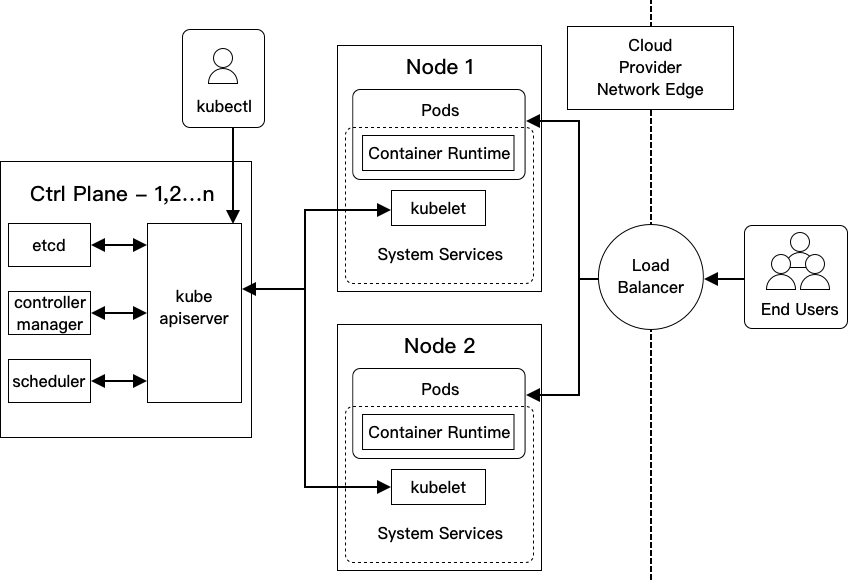
\includegraphics[width= 1\textwidth]{pics/Kubernetes-architecture.png}\\
  \caption{Kubernetes架构图}\label{fig:k8s-arch}
\end{figure}

\paragraph{节点}
Kubernetes集群中的主机称为节点,可以是虚拟机,也可以是物理机。一个节点有以下信息\cite{k8sconcepts}。

\begin{itemize}
	\item \textbf{Address},由主机名、机器的外部IP和集群中的内部IP组成。
	\item \textbf{Capacity和Allocatable},描述了节点的CPU、内存和存储边界,以及可以在其上部署多少进程。
	\item \textbf{Conditions},例如“Ready”状态,“NetworkUnavailable状态”以及一些关于节点压力的信息:“MemoryPressure”会对内存占用率过高的情况发出警告;“DiskPressure”会对硬盘占用率过高的情况发出警告;“PIDPressure”会对该节点上分配的进程过多的情况发出警告。这些标志会根据节点当前的实际状态进行更新。
	\item \textbf{Info},描述了节点的一般信息,如内核版本、Kubernetes版本、Docker版本(如果使用)和操作系统名称。
\end{itemize}

\paragraph{主节点}
主节点充当集群的网关和大脑,将API暴露给用户使用从而与Kubernetes交互。主节点是Kubernetes集群的入口,负责Kubernetes提供的大部分中心化逻辑。它决定了如何调度任务,即如何将工作分割和分配给节点。它还收集节点的日志和健康状态。主节点通常专门负责编排容器,而节点则负责实际的运行容器。

在高可用性集群中,多个主节点被实例化,以实现冗余备份,目的是在低于一定数量的主节点故障的情况下也能保证集群的运行\cite{ha}。

\subsection{Kubernetes控制面}
如图\ref{fig:k8s-ctrl}所示,Kubernetes控制面由运行在主节点上的各种组件组成。

\paragraph{etcd}
etcd对于Kubernetes跨节点工作至关重要,因为它提供了一个轻量级和分布式的键值存储,可以跨越多个节点。Kubernetes使用etcd来存储配置数据,这些数据可以被集群中的每个节点访问。它通常安装在主节点上,在生产系统和高可用性集群中,安装在多个主节点上,以实现冗余和弹性。

\paragraph{kube-apiserver}
kube-apiserver是整个集群的主要控制模块。所有的管理工具,包括Kubernetes命令行工具kubectl,都是通过它暴露的那些API与Kubernetes进行通信的。 kubectl是默认的从本地计算机与Kubernetes集群交互的方法,允许管理集群、部署及管理Kubernetes对象。

\begin{figure}[htbp]
  \centering
  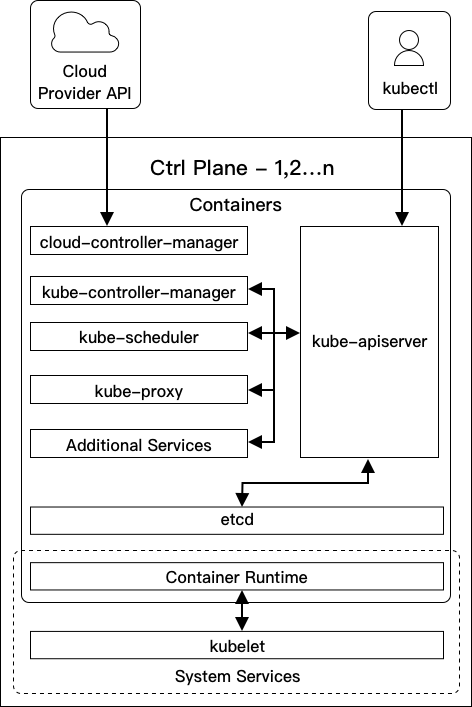
\includegraphics[width= 1\textwidth]{pics/K8s-ctrl-plane.png}\\
  \caption{Kubernetes控制面\cite{gorillaguide}}\label{fig:k8s-ctrl}
\end{figure}

\paragraph{kube-scheduler}
kube-scheduler是一个通过分析当前基础设施环境将工作负载分配给节点的服务。为此,它需要跟踪每台主机上的可用容量,以确保工作负载不会超过某个节点或整个集群上的可用资源\cite{introk8s}。

\paragraph{kube-controller-manager}
kube-controller-manager是一个具有许多职责的通用服务,可以将其视为控制器组件的集合。这其中的每一个控制器都会调节集群的状态,管理工作负载生命周期,或者执行常规任务\cite{gorillaguide}。

当检测到一个变化时,控制器读取新的信息并执行满足所需状态的程序。这可能涉及到扩大或缩小应用程序的规模,调整端点等。例如,ReplicaSet确保为一个应用程序定义的副本数量与当前部署在集群上的数量相匹配。

\paragraph{cloud-controller-manager}
Kubernetes可以部署在许多不同的环境中,例如,裸机服务器、AWS(Amazon Web Services)、GKE(Google Kubernetes Engine)、Azure等等。每一种服务都有不同的API和Kubernetes对象的实现。Kubernetes必须与这各种各样的基础设施和云提供商进行交互,将它们的非同质资源映射到其资源抽象中。cloud-controller-manager作为Kubernetes和底层基础设施之间的粘合剂。它告诉Kubernetes如何与目标基础设施的不同能力、特性和API进行交互。由于一个Kubernetes可能同时分布在多个环境中,所以在一个集群中可以有多个cloud-controller-manager,每个环境都有一个。

\subsection{节点服务组件}
Kubernetes控制面只需要部署在主服务器上,同时一些组件也必须安装在每个节点上,图\ref{fig:k8s-node}展示了这些组件。

\paragraph{容器运行时}
容器运行时负责启动和管理容器。Docker是典型的容器运行时,同时还有很多其他的选择,例如podman、containerd等,云提供商也可以提供自己定制的容器运行时来满足这一组件要求。

\begin{figure}[htbp]
  \centering
  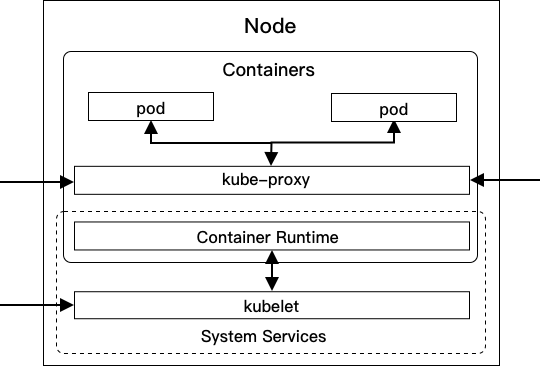
\includegraphics[width= 1\textwidth]{pics/K8s-node-server-components.png}\\
  \caption{Kubernetes节点服务组件\cite{gorillaguide}}\label{fig:k8s-node}
\end{figure}

\paragraph{kube-proxy}
kube-proxy负责在节点之间创建网络,从而让节点加入Kubernetes集群接收流量。它还将传入节点的请求转发到正确的容器,也实现了一些基本形式的负载均衡。另外,它确保每个网络环境的正确隔离。

\paragraph{kubelet}
Kubelet负责与控制面服务交换信息。它从主节点组件接收命令和任务。任务以manifest的形式接收,manifest定义了要部署的资源和操作参数。在接收到一堆任务后,kubelet会负责执行工作和维护节点服务器上相关资源,一切都通过与容器运行时的交互来完成。

\subsection{Kubernetes对象}
Kubernetes对象也被叫做资源(resources),Kubernetes自身定义了一组构件,提供了部署、维护和扩展应用的机制,这些构件都是“Kubernetes native resources”。这些基元可以通过Kubernetes API进行扩展,基于这一点Kubernetes Operators才可以实现。利用Kubernetes扩展性实现的工具可以作为Kubernetes容器运行,方便相关应用的部署与管理。

\paragraph{Spec和Status}
几乎每一个Kubernetes对象都包括两个嵌套的对象字段,用来管理该对象的配置,即对象规格(spec)和对象状态(status)。规格描述了对象的期望状态,而其状态则描述了当前的状态。Kubernetes不断地对对象进行操作,目标是最终让当前状态与spec中给出的期望状态相匹配。

\paragraph{Pod}
Pod是Kubernetes中的基本部署单元,也是最小单元。一个Pod就是一群鲸鱼的社会群体\cite{k8sconcepts}。这个比喻很形象:Kubernetes Pod是一组容器化组件的抽象。一个或多个紧密耦合的容器被封装在一个对象中,保证它们在同一台主机上被共同定位和调度,并且可以共享资源。

Pod中的容器紧密地运行在一起,共享一个生命周期,并且总是被调度到一个节点上。Kubernetes将它们作为一个单元进行管理,它们共享环境、卷和IP空间。Pod中的所有容器都可以在localhost上相互引用,正因为如此,Pod中的应用必须协调它们对端口的使用。一个容器的暴露端口也会从Pod中暴露出来。从容器外部,无法与Pod中的某个容器进行通信,我们只能与Pod进行通信,从而到达相应端口的容器。

\begin{figure}[htbp]
  \centering
  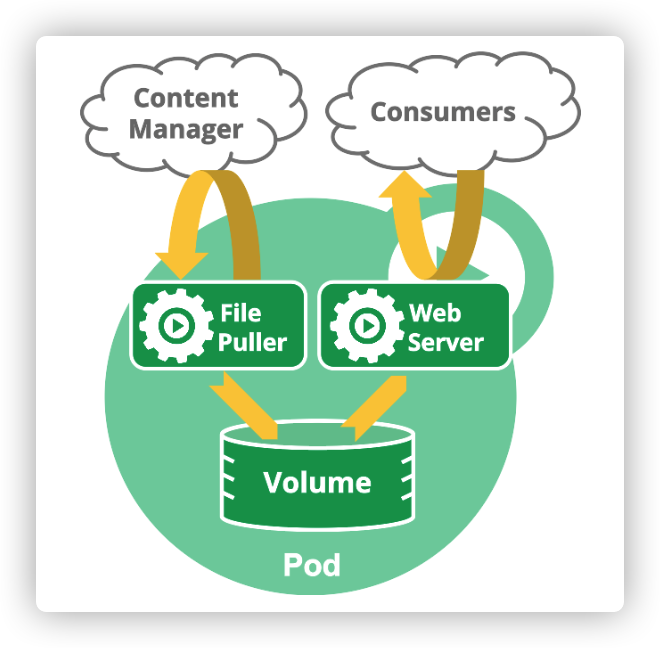
\includegraphics[width= 1\textwidth]{pics/pod.png}\\
  \caption{Pod示例}\label{fig:pod}
\end{figure}

像容器一样,Pods被认为是相对短暂的实体,而不是持久的。Pod的唯一标识符(UID)和IP会一直保持到Pod终止。终止可能发生在用户发送终止命令时(有宽限期),宽限期结束时,新的版本被部署,旧的Pod在过渡期后被认为是死亡的。当Pod内的命令终止时,Pod也会死亡\cite{k8sconcepts}。

通常情况下,Pods由一个满足工作目的的主容器和一些帮助容器(称为sidecars)组成,这些容器可以帮助完成密切相关的任务。这些程序在自己的容器中运行,但与主应用程序紧密相连\cite{introk8s}。例如,一个要在后台运行的周期性任务,如图\ref{fig:pod}中的“File Puller”,它负责与远端同步数据,而“Web Server”作为主服务器启动一个Web服务供用户访问查看这些数据,他们使用同一个volume,从而共享其中存储的文件。

因此,在一个Pod中运行多个容器与在一个容器中运行多个程序是完全不同的,即可以达到在localhost上拥有多个程序的所有优点,同时获得透明度、软件依赖性的解耦、效率和易用性。水平缩放不应该在Pod内部通过容器增减实现,而应该在外部,缩放Pod\cite{k8sconcepts}。

\paragraph{Volume}
Kubernetes Volume是存储的一个抽象。容器中的磁盘文件是短暂的,因为它们与容器一起死亡,当一个新的容器被部署时,它将从原始映像的干净状态开始。这可能会对有状态的应用程序造成问题,例如,存储系统或数据库。此外,有时在Pod中一起运行的容器需要共享文件。Volume的抽象解决了这两个问题。

Volume也不是完全持久化的。当一个Pod被移除时,相关的Volumes也会随之被销毁。Kubernetes Persistent Volumes避免了这一问题,它是一种抽象化的机制,它可以抽象出更强大的存储,不与Pod的生命周期挂钩\cite{k8sconcepts}。Persistent Volumes是集群的独立存储资源,可以通过“PersistentVolumeClaim”连接到Pod上。如果Pod被移除,持久化卷就会被释放而不会被删除。这样就可以将之前的存储重新连接到新版本的Pod上,恢复其数据。

\paragraph{ReplicaSet}
ReplicaSet的目的是维持一组稳定的副本Pod的正确运行。因此,它经常被用来保证指定数量的相同Pod的可用性\cite{k8sconcepts}。ReplicaSet通过根据需要创建和删除Pod来实现其目的,以达到期望的副本数量。当ReplicaSet需要创建新的Pod时,它使用ReplicaSet spec中的Pod模板来配置Pod。

ReplicaSet 部署的所有Pod都会通过“ownerReference”字段链接到它。这帮助ReplicaSet知道它正在维护的Pod的数量和种类,从而去决定应该创建一个新的Pod,还是删除其中一个现有的Pod。有一种情况是一个Pod没有所有者参考,可能是因为它是用户手动创建的,但它符合ReplicaSet的选择器,它将立即被获取,设置“owerReference”字段为该ReplicaSet。

\paragraph{Deployment}
Deployment为 Pods 和 ReplicaSets 提供声明式更新\cite{k8sconcepts}。Deployment是一种高级别对象,旨在简化副本pods的生命周期管理。一个Deployment描述了期望的状态,Deployment Controller以可控的速度将实际状态改变为期望状态。Deployment可以修改目标配置,Kubernetes会调整ReplicaSet,管理不同应用版本之间的过渡。

\paragraph{Service}
如图\ref{fig:service}所示,Service是一种将运行在一组Pod上的应用作为网络服务公开的抽象方式\cite{k8sconcepts}。一个Kubernetes Service也可以作为pods的内部负载平衡器。它将执行相同功能的pods收集在一起作为一个逻辑集合,使其呈现为一个单一实体,并在它们之间路由传入流量。一个Pod是否应该加入Service的集合由标签选择器定义。

\begin{figure}[htbp]
  \centering
  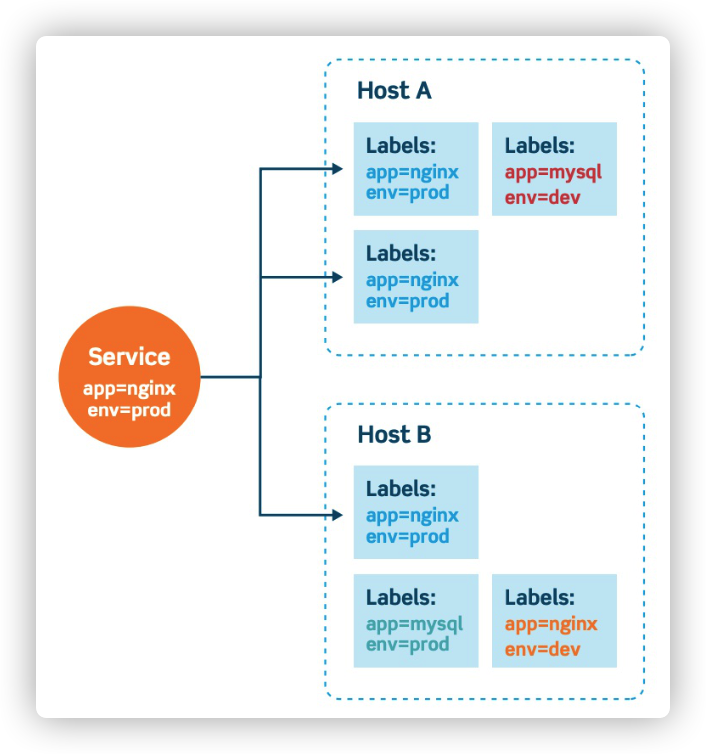
\includegraphics[width= 1\textwidth]{pics/service.png}\\
  \caption{Service标签示例\cite{gorillaguide}}\label{fig:service}
\end{figure}

Service为非持久化的对象提供了一个稳定的端点。Service允许根据需要扩展或替换后端单元。同时,无论它路由到的Pod集合如何变化,Service的IP地址都会保持稳定\cite{introk8s}。通过部署Service,应用可以轻松获得可发现性,并可以简化容器设计。

Service资源会收到一个ClusterIP,仅在内部IP上暴露服务\cite{gorillaguide}。这使得服务只能从集群内部到达。NodePort在每个节点的IP上通过指定的端口暴露服务。这个功能允许设置一个外部负载平衡器,或者在需要的时候,在其特定的端口上暴露应该从外部世界可达的服务。更多的时候,NodePorts用于调试目的,以快速的方式暴露服务,避免在开发的第一阶段配置路由或Ingresses。

\paragraph{ConfigMap}
ConfigMap也是一个Kubernetes对象,用于在键值对中存储非机密数据。Pods可以将ConfigMaps作为环境变量、命令行参数或卷中的配置文件来使用。ConfigMaps允许将特定环境的配置从容器镜像中解耦出来,从而使应用程序易于移植。

\section{Kubernetes Operators}
Kubernetes官方文档将Operators描述为“Kubernetes的软件扩展,利用自定义资源来管理应用程序及其组件”\cite{k8soperator}。一个Operator本质上就是一个自定义资源类型和一个监视该资源类型并做出实际操作的自定义控制器的组合。控制器是Kubernetes中的一个核心概念,它被实现为一个控制循环,在Kubernetes中的一个Pod内持续运行,如图\ref{fig:reconciliation-loop}所示,它比较对象的期望状态和当前状态,并在需要时随时调和这种状态。事实上,当对象的当前状态与期望状态不同时,管理Kubernetes Operator会对对象发出指令,使其最终达到期望状态。

\begin{figure}[htbp]
  \centering
  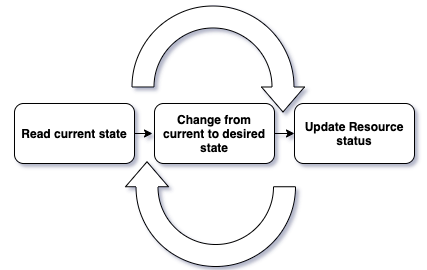
\includegraphics[width= 1\textwidth]{pics/reconcile-loop.png}\\
  \caption{控制循环}\label{fig:reconciliation-loop}
\end{figure}

一个Operator是一个运行在集群上的Pod中的软件,与Kubernetes API服务器交互。它通过CustomResourceDefinition(Kubernetes中的一种扩展机制)引入新的对象类型。Operator监控这种自定义资源类型,并被通知其存在或修改。当Operator收到这种通知时,它将开始运行一次循环,以确保这些对象所代表的应用服务的所有所需连接实际上是可用的,并按照用户在对象spec中表达的方式进行配置。例如,Grafana Operator将Grafana和GrafanaDashboard对象添加到Kubernetes中。希望部署Grafana的用户只需要创建一个Grafana对象,并将其所需配置作为参数填入自定义资源spec中。Operator将部署所有必要的对象并保持其运行。

\subsection{kubebuilder与Operator SDK}
kubebuilder和Operator SDK都是Operator的开发工具。kubebuilder由kubernetes特别兴趣小组(sigs)推出,而Operator SDK由CoreOS推出,它们的功能非常接近,在稍早的版本中,它们生成的Operator项目框架和底层依赖会有些区别,但是现在已经达成合作,二者同质化,这里就一起介绍了。

它们都只为Go开发者服务,都相当依赖于代码生成器,都提供了一个命令行工具来创建一个新项目、生成代码、构建二进制文件、镜像、配置清单等,都把控制器模式作为一个库来实现。

它们的功能都很强大,但是缺点也很明显:
\begin{itemize}
	\item 限定编程语言,提高了使用门槛,Go语言有很多对新手不友好的地方。
	\item 本质上是代码生成工具,但是版本兼容性较差,不同的版本对应不同的Kubernetes版本,但是旧版本生成的项目必须手动升级成新版本项目,没有自动化工具。
	\item 用户依然要学习使用Kubernetes客户端库,用指令式代码与Kubernetes交互,编写旧版本资源向新资源迁移的代码,处理新旧资源的合并。
\end{itemize}

\section{Serverless}
随着以 Kubernetes 为代表的云原生技术成为云计算的容器界面,Kubernetes 成为云计算的新一代操作系统。面向特定领域的后端云服务(BaaS)则是这个操作系统上的服务 API,存储、数据库、中间件、大数据、AI 等领域的大量产品与技术都开始提供全托管的云形态服务,如今越来越多用户已习惯使用云服务,而不是自己搭建存储系统、部署数据库软件。

当这些 BaaS 云服务日趋完善时,Serverless 因为屏蔽了服务器的各种运维复杂度,让开发人员可以将更多精力用于业务逻辑设计与实现,而逐渐成为云原生主流技术之一。Serverless 计算包含以下特征:

\begin{itemize}
	\item \textbf{全托管的计算服务},客户只需要编写代码构建应用,无需关注同质化的、负担繁重的基于服务器等基础设施的开发、运维、安全、高可用等工作。
	\item \textbf{通用性},结合云 BaaS API 的能力,能够支撑云上所有重要类型的应用。
	\item \textbf{自动的弹性伸缩},让用户无需为资源使用提前进行容量规划。
	\item \textbf{按量计费},让企业使用成本得有效降低,无需为闲置资源付费。
\end{itemize}

函数计算(Function as a Service)是 Serverless 中最具代表性的产品形态。通过把应用逻辑拆分多个函数,每个函数都通过事件驱动的方式触发执行,例如当对象存储(OSS)中产生的上传 / 删除对象等事件, 能够自动、可靠地触发 FaaS 函数处理且每个环节都是弹性和高可用的,客户能够快速实现大规模数据的实时并行处理。同样的,通过消息中间件和函数计算的集成,客户可以快速实现大规模消息的实时处理。

Serverless计算与容器技术结合后诞生出了更多其他形式的服务形态。通过良好的可移植性,容器化的应用能够无差别地运行在开发机、自建机房以及公有云环境中; 基于容器工具链能够加快解决 Serverless 的交付。云厂商如阿里云提供了弹性容器实例(ECI)以及更上层的 Serverless 应用引擎(SAE),Google 提供了 CloudRun 服务,这都帮助用户专注于容器化应用构建,而无需关心基础设施的管理成本。此外 Google 也开源了基于 Kubernetes 的 Serverless 应用框架 Knative。Bitnami也开源了kubeless,一个轻量易用的serverless框架。kubeless是本文后续主要使用的工具之一,用于将用户编写的自定义调谐函数部署成一个web服务。

\section{小结}
本章主要介绍了UniversalController开发过程中所使用的相关技术以及使用技术的场景。首先介绍了容器化技术,这是如今云上应用的默认部署方式。然后介绍了容器编排系统Kubernetes,它是实际的业界标准,接着介绍Kubernetes Operator这一Kubernetes上的重要概念与拓展方式,介绍了现有的开发工具已经开发中存在的问题。最后简要介绍了基于UniversalController开发Operator时会用到的serverless技术。

%%%%%%%%%%%%%%%%%%%%%%%%%%%%%%%%%%%%%%%%%%%%%%%%%%%%%%%%%%%%%%%%%%%%%%%%%%%%%%%
\chapter{声明式的通用Kubernetes Operator的需求分析与设计}\label{chapter_framework}
本文所陈述的声明式的通用Kubernetes Operator,即UniversalController,主要是为了让开发者更容易的去实现以及部署Kubernetes Operators,进而扩展Kubernetes的API。

\section{需求分析}

\subsection{事件配置}
首先,UniversalController应该能够方便简明地通过配置指明调谐过程应该被那些事件源触发。在Kubernetes上实现自定义调谐的主要方法是将特定域的期望状态封装在一个或多个自定义资源中,由自定义控制器来监视并执行调谐。

出于这个原因,UniversalController的监视配置功能应该允许用户初始化这个资源监视过程。为了最大限度地减少模板代码,配置接口应该尽量最小化,只需要特定于应用程序的必要参数,例如要监视的(自定义)资源的基本信息(apiVersion和kind)。

例如,开发人员在构建TensorflowJob Operator时,应该能够简单地指示UniversalController监视所有TensorflowJob类型的资源的事件。

\subsection{支持动态资源类型}
作为一个通用Operator,UniversalController事先不能知道它要处理哪些种类的资源。需要处理的是K8s内部定义的原生资源还是用户自定义资源,这些在实现时都是未知数,只有在运行时才能知道,所以UniversalController需要支持动态资源类型,能够处理Kubernetes系统内任意一种资源。

\subsection{易用的调谐接口}
调谐逻辑是Kubernetes Operators的核心部分和价值,所以开发者还要能够轻松地提供以业务逻辑为中心的自定义调谐函数。

当实现调谐函数时,开发人员应该能够专注于自定义的业务逻辑,同时尽量减少需要编写和理解的底层Kubernetes或UniversalController特定逻辑。

因此,UniversalController应该提供一个编程接口,用于接受自定义的调谐函数,它将与所提供的事件配置自动匹配。此外,为了让开发者编写代码时作出正确的决策,UniversalController应该将上下文信息,如事件元数据,暴露给自定义代码。最后,开发者提供的代码还应该能够根据调谐的结果指导下一步的行动。

\subsection{多控制器并存}
当开发一些项目时,可能需要在一个进程中打包并部署多个自定义控制器,例如kube-controller-manager和cloud-controller-manager组件都是这样工作的。

在这种情况下,依然需要保持关注点的分离,使用具有不同配置的单独控制器来调谐不同的Kubernetes Resources。但控制器的集合确实构成了一个便于协作的单元自动化服务,并且还可以共享一些Kubernetes特定的配置,如认证、订阅等。

因此,UniversalController的另一个需求是支持这样的配置,允许定义和运行多个控制器。

\subsection{降低工作量}

\begin{figure}[htbp]
  \centering
  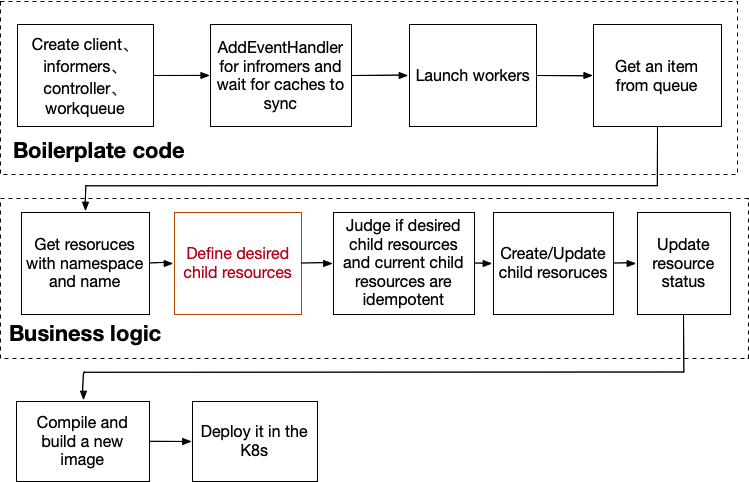
\includegraphics[width= 1\textwidth]{pics/coding-operator.png}\\
  \caption{Operator编写流程}\label{fig:coding-operator}
\end{figure}

图\ref{fig:coding-operator}是一个Operator开发的基本流程。UniversalController需要能够对此进行简化,舍去或简化一些步骤。就像一个Operator简化了某个应用的部署、更新与管理,UniversalController需要能简化一个controller的开发、创建与管理。

\subsection{语言无关}
Kubernetes本身是用Go语言开发的,因此官方也推荐用Go来开发Operator,可以使与Kubernetes APIs的集成更简单。Kubernetes的Go客户端clieng-go也确实是最古老且最成熟的,得到了完善的测试并且可靠,Kubernetes组件内部也会使用它。而基于client-go的controller-runtime提供了更高级的抽象,让Operator的开发更加便利。但是其他编程语言则没有那么可靠成熟的Operator开发工具,比如Python和Java虽然有Kubernetes官方团队推出的客户端,但是都只提供了低级的抽象,用来实现Operator会显得极为繁琐。

针对这种现象,UniversalController被设计成语言无关的,只要开发者使用的编程语言能够理解json就可以用来编写Operator。

\subsection{通用性}
UniversalController对一般的Operator做了一层高级的抽象,但是同时也需要保留充分的灵活性,以确保它能够适用于大部分情况,用户得到的应该是一种通用的开发方式。


\section{设计}
UniversalController自身也是一个Kubernetes Operator,负责监视UniversalController CRD(下文简称UC CRD)并维护它们对应的自定义控制器。创建一个新的UC CRD等同于在系统中注册一个新的自定义控制器。Kubernetes提供的动态API注册机制CustomResourceDefinition,这让用户可以声明式地创建一种新的自定义资源,UniversalController扩展了Kubernetes的API,UC CRD接口进一步让用户可以声明式地创建自定义控制器。

\subsection{总体架构}

\begin{figure}[htbp]
  \centering
  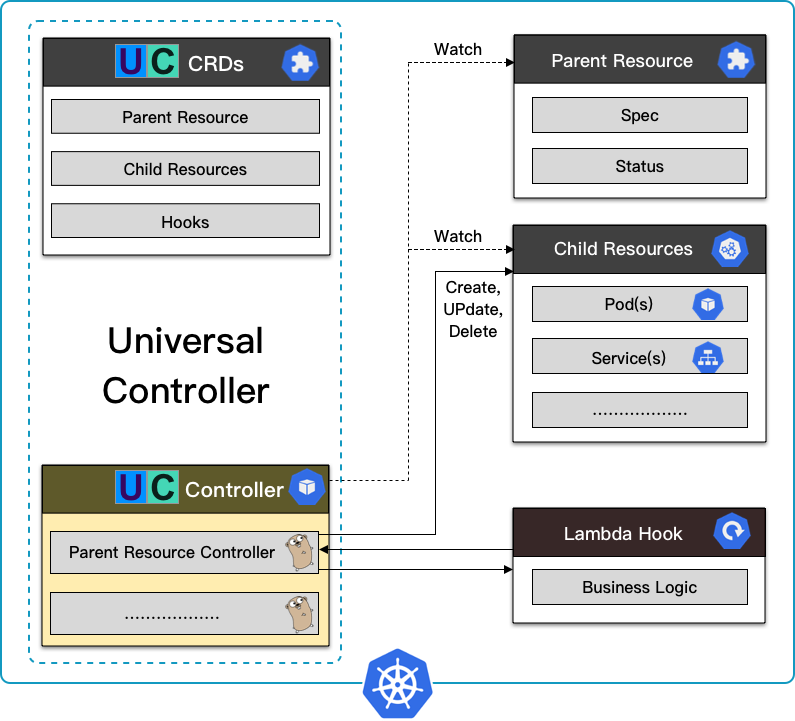
\includegraphics[width= 1\textwidth]{pics/uc-arch.png}\\
  \caption{UniversalController架构}\label{fig:uc-arch}
\end{figure}

图\ref{fig:uc-arch}展示了UniversalController的总体架构。UniversalController自身是一个Kubernetes中的controller,负责监视UniversalController CRDs,当有一个新的UniversalController CRD被创建时,它会启动Parent Resource的控制器作为响应。也就是说,UniversalController是控制器的控制器,可以用于管理多个控制器,实现多控制器并存在一个进程中运行。

\subsection{自定义资源}

UC CRD是UniversalController提供的声明式API,通过Kubernetes CustomResourceDefinition注册在Kubernetes API中。通过创建一个UC资源,可以很方便的定制一种控制器,它根据父对象中指定的期望状态管理一组子对象,这也是最常见的控制器类型。像Deployment、StatefulSet、TFJob、PytorchJob的控制器都是符合这种模式的。

UC CRD是对控制器的高级抽象,包含了一个控制器运行时需要知道的各项信息,例如事件配置、更新策略和调谐接口访问地址。

\begin{itemize}
	\item 用户只需要填写好parentResource对象和childResources对象数组,UniversalController就会对这些资源进行监视,订阅它们的相关事件。
	\item childResources对象数组中的每个childResource对象都有一个updateStrategy对象,通过设置它实现声明式的更新策略,支持OnDelete, Recreate, InPlace, RollingRecreate, RollingInPlace。
	\item 调谐接口是唯一需要用户编码实现的模块,用户在这里只需要关心实际业务逻辑,开发完成后将其部署成一个web服务,将服务地址填入UC CRD的相应字段即可。
\end{itemize}

\subsection{动态类型资源处理}
Kubernetes的官方Go语言客户端库client-go,提供了dynamic模块,可以用于创建动态客户端,借助于动态客户端,只要知道资源的apiVersion和Kind,就可以对任意一种资源进行操作。UniversalController基于此,实现了支持动态资源类型的informer和indexer,用于订阅特定资源相关事件以及查找特定类型的资源,是自定义控制器的核心组件。

\subsection{控制器设计}\label{controllerdesign}


\begin{figure}[htbp]
  \centering
  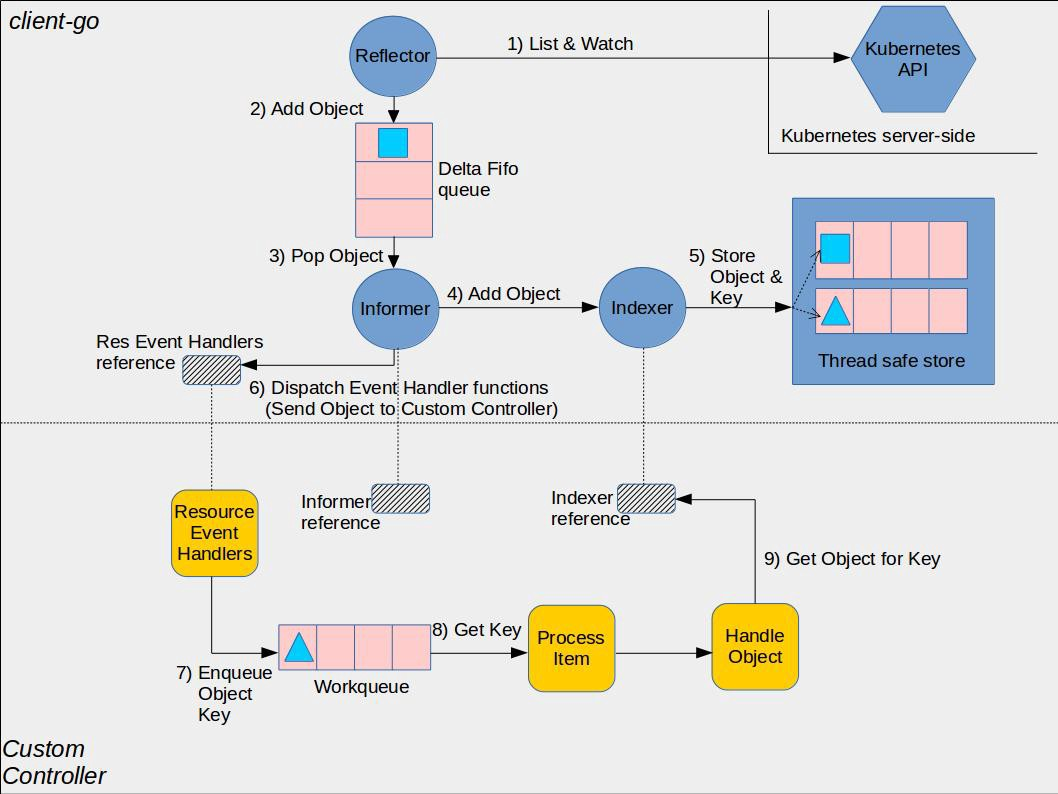
\includegraphics[width= 1\textwidth]{pics/client-go-controller-interaction.jpeg}\\
  \caption{controller工作原理\cite{controllerclientgo}}\label{fig:client-go-controller}
\end{figure}

图\ref{fig:uc-arch}中的UC Controller和Parent Resource Controller都是自定义控制器。图\ref{fig:client-go-controller}展现了一个自定义控制器的工作方式。

首先介绍一下client-go提供给开发者的组件:
\begin{itemize}
	\item \textbf{反射器(Reflector)}:反射器监视着Kubernetes API中的指定资源类型(Kind)。完成这项工作的方法(function)是“ListAndWatch”。监视的对象可以是内置的原生资源,也可以是自定义资源。当反射器通过监视API收到有新资源诞生的通知时,它使用相应的listing API获得该对象,调用“watchHandler”方法,将其放入“Delta FIFO”队列中。
	\item \textbf{通知器(Informer)}:通知器从“Delta FIFO”队列中弹出对象。它的工作是保存对象以便以后检索,并向自定义控制器传递对象。
	\item \textbf{索引器(Indexer)}:索引器提供索引对象的功能。一个典型的索引用例是基于对象标签创建索引。索引器可以基于几个索引功能来维护索引。索引器使用一个线程安全的数据存储来存储对象和它们的键。默认会使用Store类型中一个名为MetaNamespaceKeyFunc的方法来生成键,该方法将一个对象的键生成为该对象的<命名空间>/<名称>组合。
\end{itemize}

而自定义控制器中有一下组件:
\begin{itemize}
	\item \textbf{资源事件处理器(Resource Event Handlers)}:资源事件处理器是回调函数,当通知器(Informer)向控制器传递一个对象时,它将被调用。编写这些函数的典型模式是获取被传递对象的键,并将该键排入工作队列(workqueue)等待进一步的处理。
	\item \textbf{工作队列(Workqueue)}:工作队列将对象的传递与处理脱钩,接受到对象后不会立即处理而是放入队列中。
	\item \textbf{处理程序(Process Item)}:处理程序被用于处理工作队列中的项目,它通常使用索引器来检索与键对应的对象。
\end{itemize}

UC Controller和Parent Resource Controller都使用这种经典控制器模式。

UC Controller监视着UC类型的资源,提供了UC相关的服务,同时管理着通过UC CRD创建的自定义控制器。它的“Handle Object”部分确保集群状态与UC CRD期望的一致,也就是保持所有注册的自定义控制器正确运行。

而Parent Resource Controller监视着Parent Resource,它的“Handle Object部分”是UniversalController用户自定义的代码段,一般是若干个函数。

当开发者使用UC的声明式API创建控制器时,开发者需要提供的函数中只包含当前控制器所特有的业务逻辑。这些函数会通过webhook调用,所以开发者可以用任何能够处理网络请求和JSON的编程语言来编写这些函数。

Parent Resource Controller会执行一个调谐循环,在调谐时调用开发者提供的函数,之后再决定做什么。UniversalController为每一个Parent Resource Controller预先准备了调谐循环的通用逻辑,开发者不需要借助代码生成器,可以完全将精力集中在编写调谐函数上。现阶段UniversalController接受的调谐器是Webhook形式的,开发者可以借助serverless工具,例如kubeless或者openFaas,将函数发布成一个Web服务,再提供给控制器。借助UC的API和serverless就可以使开发工作完全集中于业务逻辑,免去了很多琐碎的工作和模版代码。

\subsection{声明式的调谐器}
图\ref{fig:uc-arch}中的“Lambda Hook”模块就是UniversalController中的调谐器,以webhook的形式实现。

调谐器的工作本质上其实就是两个翻译过程:
\begin{itemize}
	\item 根据集群的当前状态(state)更新资源的状态(status)。
	\item 根据资源的specification对Kubernetes集群进行操作,一般是编排一些Kubernetes原生资源,例如Pods、Services等,来完成某个应用(例如数据库)的部署与维护。
\end{itemize}

\begin{figure}[htbp]
  \centering
  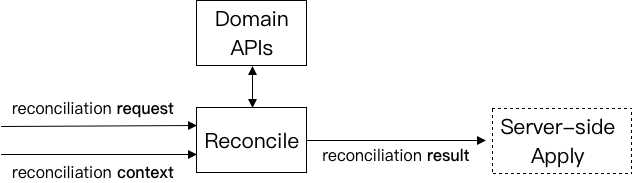
\includegraphics[width= 1\textwidth]{pics/reconciler-interface.png}\\
  \caption{调谐器}\label{fig:reconciler}
\end{figure}

图\ref{fig:reconciler}是一般的调谐器抽象,它接受调谐请求和当前系统上下文,并返回调谐的结果。在Kubernetes中Domain APIs就是各种资源,包括Pod、Service、ReplicaSet等,用户自定义的资源也包含在其中。在UC中,调谐请求就是当前被处理的资源对象,上下文就是通过标签筛选出的子资源以及相关资源,调谐结果是根据当前状态(state)得到该资源对象的状态(status)以及根据该资源对象的规格(specification)得到的期望子资源。

基于UniversalController编写的调谐器不用去处理资源的增删改查,不用去与Kubernetes交互,只需要去返回期望状态(期望存在的资源集合)。UC Controller会去决定怎么到达期望状态。这个过程与用户直接通过kubectl将资源描述文件提交给api-server很接近,指令式的操作极少,也是声明式的。

UniversalController使用自己的服务端应用(server-side apply)逻辑,它与“kubectl apply”的逻辑接近,遵循惯例而不是配置。开发者不需要在CRD中提供如何合并旧资源与新资源的提示,它们的自定义资源和原生资源都根据一套“apply”逻辑得到合并结果。

现阶段调谐器需要以Webhook的形式提供,任何可以编写网络服务并处理json的编程语言都可以用于编写这段核心业务逻辑。这是实现语言无关特性的关键。借助serverless工具,开发者实际需要编写的只是一个函数而已,其lambda表达式为(parent, children, related) => \{... return (status, children)\}。

\newpage
\begin{lstlisting}[language=Go,caption=sample-controller中对资源进行增删改查的代码段,label=listing:crud-rc]
foo, err := c.foosLister.Foos(namespace).Get(name)
deployment, err := c.deploymentsLister.Deployments(foo.Namespace).Get(deploymentName)
if errors.IsNotFound(err) {
    deployment, err = c.kubeclientset.AppsV1().Deployments(foo.Namespace).Create(context.TODO(), newDeployment(foo), metav1.CreateOptions{})
}
if foo.Spec.Replicas != nil && *foo.Spec.Replicas != *deployment.Spec.Replicas {
    deployment, err = c.kubeclientset.AppsV1().Deployments(foo.Namespace).Update(context.TODO(), newDeployment(foo), metav1.UpdateOptions{})
}
_, err := c.sampleclientset.SamplecontrollerV1alpha1().Foos(foo.Namespace).Update(context.TODO(), fooCopy, metav1.UpdateOptions{})
\end{lstlisting}

\subsection{声明式的更新策略}
Kubernetes的原生资源Deployment和StatefulSet都有对它们管理的Pod进行滚动更新的功能。UniversalController也支持滚动更新,内置了多个可选的更新策略,并且可以通过声明式使用,开发者只需要在UC资源中填入相应字段就可以让自己的控制器拥有滚动更新的能力。

\section{小结}

本章首先对一个通用Opeator需要实现的功能进行了介绍,然后在需求分析的基础之上对UniversalController的总体架构和各个模块进行了详细说明。

%%%%%%%%%%%%%%%%%%%%%%%%%%%%%%%%%%%%%%%%%%%%%%%%%%%%%%%%%%%%%%%%%%%%%%%%%%%%%%%
\chapter{声明式的通用Kubernetes Operator的实现}\label{chapter_implement}
UnversalController自身依然是一个传统的Operator,用Go语言编写完成。因为UniversalController不能事先确定自己需要监视和处理的资源类型,所以使用了Kubernetes官方Go语言客户端client-go的dynamic包,它提供了动态的客户端,可以操作任意类型的资源,包括原生资源以及用户自定义资源,这是它作为一个通用Operator的关键。

\section{自定义资源}

\begin{lstlisting}[language=yaml,caption=UC CRD,label=listing:1]
apiVersion: apiextensions.k8s.io/v1
kind: CustomResourceDefinition
metadata:
  annotations:
    "api-approved.kubernetes.io": "unapproved, request not yet submitted"
  name: "universalcontrollers.universalcontroller.njuics.cn"
spec:
  group: "universalcontroller.njuics.cn"
  names:
    kind: UniversalController
    listKind: UniversalControllerList
    plural: universalcontrollers
    shortNames:
    - uc
    - uctl
    singular: universalcontroller
  scope: Cluster
...
\end{lstlisting}

YAML代码\ref{listing:1}是UC CRD的定义,通过kubectl向api-server提交这个yaml文件就可以在Kubernetes中注册一种新的资源类型“UniversalController”。这样就成功拓展了Kubernetes APIs,之后就可以使用这个新的API提交资源定义来注册控制器。

\begin{lstlisting}[language=yaml,caption=作为UC CRD示例的catset-controlelr,label=listing:ucsample]
apiVersion: universalcontroller.njuics.cn/v1alpha1
kind: UniversalController
metadata:
  name: catset-controller
spec:
  parentResource:
    apiVersion: mlhub.njuics.cn/v1alpha1
    resource: catsets
  childResources:
    - apiVersion: v1
      resource: pods
      updateStrategy:
        method: RollingRecreate
        statusChecks:
          conditions:
            - type: Ready
              status: "True"
    - apiVersion: v1
      resource: persistentvolumeclaims
  hooks:
    sync:
      webhook:
        url: "http://catset-ctrl.universalcontroller:8080"
\end{lstlisting}

YAML文件\ref{listing:ucsample}是一个UC CRD资源的例子,定义了CatSet资源的控制器,它的行为几乎与Kubernetes原生资源的StatefulSet的控制器一致,是对StatefulSet的二次实现。

一个UC CRD的“spec”有如下字段:

\begin{itemize}
	\item parentResource:类型是ResourceRule,用于指定父资源类型,也就是这个控制器实际管理的资源。ResourceRule只有两个字段“APIVersion”和“Resource”,用于确定一种资源类型。
	\item childResources:是一组ResourceRule,用于指定会被控制器生成的子资源类型。
	\item resyncPeriodSeconds:规定两次调谐之间间隔的时间,设置后就算工作队列当前是空的,但是距离上次调谐过去这么多时间后还是会去调谐。
	\item generateSelector:bool型,如果为真,那么忽略父资源对象的标签选择器(如果存在的话),UniversalController会为其生成独一无二的标签选择器,避免与其他的资源冲突。这里的标签选择器都是为了筛选子资源,符合标签选择器的子资源都会被当做父资源的子资源。
	\item hooks:一组定义了控制器行为的lambda hook。
\end{itemize}

\section{动态类型高级操作接口实现}

\begin{lstlisting}[language=Go,caption=客户端实现,label=listing:client]
type Clientset struct {
	config    rest.Config
	resources *dynamicdiscovery.ResourceMap
	dc        dynamic.Interface
}
type ResourceClient struct {
	dynamic.ResourceInterface
	*dynamicdiscovery.APIResource
	rootClient dynamic.NamespaceableResourceInterface
}
func New(config *rest.Config, resources *dynamicdiscovery.ResourceMap) (*Clientset, error)
func (cs *Clientset) Resource(apiVersion, resource string) (*ResourceClient, error) {
	// Look up the requested resource in discovery.
	apiResource := cs.resources.Get(apiVersion, resource)
	if apiResource == nil {
		return nil, fmt.Errorf("discovery: can't find resource %s in apiVersion %s", resource, apiVersion)
	}
	return cs.resource(apiResource), nil
}
func (cs *Clientset) resource(apiResource *dynamicdiscovery.APIResource) *ResourceClient {
	client := cs.dc.Resource(apiResource.GroupVersionResource())
	return &ResourceClient{
		ResourceInterface: client,
		APIResource:       apiResource,
		rootClient:        client,
	}
}
func (rc *ResourceClient) AtomicUpdate(orig *unstructured.Unstructured, update func(obj *unstructured.Unstructured) bool) (result *unstructured.Unstructured, err error)

type Unstructured struct {
	// Object is a JSON compatible map with string, float, int, bool, []interface{}, or
	// map[string]interface{}
	// children.
	Object map[string]interface{}
}
\end{lstlisting}

代码段\ref{listing:client}是客户端的结构体和一些方法,UC首先需要用New方法得到一个Clientset类型的对象,对于各种资源,只要知道资源的apiVersion和kind,都可以用这个对象的Resource方法得到一个ResourceClient对象,该对象可以对这类资源进行各类CURD的操作,所有的资源都以Unstructured类型存储,Unstructured中只有一个字典类型的字段,实际是把资源以接近JSON的形式存储起来。

\begin{lstlisting}[language=Go,caption=通知器(Informer)实现,label=listing:informer]
// sharedResourceInformer is the actual, single informer that's shared by
// multiple ResourceInformer instances.
type sharedResourceInformer struct {
	informer cache.SharedIndexInformer
	lister   dynamiclister.Lister
	defaultResyncPeriod time.Duration
	eventHandlers *sharedEventHandler
	close func()
}
func newSharedResourceInformer(client *dynamicclientset.ResourceClient, defaultResyncPeriod time.Duration, close func()) *sharedResourceInformer {
	informer := cache.NewSharedIndexInformer(
		&cache.ListWatch{
			ListFunc: func(opts metav1.ListOptions) (runtime.Object, error) {
				return client.List(opts)
			},
			WatchFunc: client.Watch,
		},
		&unstructured.Unstructured{},
		defaultResyncPeriod,
		cache.Indexers{
			cache.NamespaceIndex: cache.MetaNamespaceIndexFunc,
		},
	)
	sri := &sharedResourceInformer{
		close:               close,
		informer:            informer,
		defaultResyncPeriod: defaultResyncPeriod,
		lister: dynamiclister.New(informer.GetIndexer(), client.GroupVersionResource()),
	}
	sri.eventHandlers = newSharedEventHandler(sri.lister, defaultResyncPeriod)
	informer.AddEventHandler(sri.eventHandlers)
	return sri
}
type ResourceInformer struct {
	sharedResourceInformer *sharedResourceInformer
	informerWrapper        *informerWrapper
}
func newResourceInformer(sri *sharedResourceInformer) *ResourceInformer {
	return &ResourceInformer{
		sharedResourceInformer: sri,
		informerWrapper: &informerWrapper{
			SharedIndexInformer:    sri.informer,
			sharedResourceInformer: sri,
		},
	}
}
\end{lstlisting}

代码段\ref{listing:informer}展示了如何在client的基础之上实现informer,informer会调用client的List和Watch方法来监听资源。SharedInformer的作用是让在一个进程中运行的控制器们共享订阅,避免重复订阅浪费内存和网络带宽。

\section{控制器实现}

一个UC CRD被提交后就相当于在UniversalController中注册了一个新的控制器。

UC Controller和Parent Resource Controller的资源事件处理器(Resource Event Handlers)、工作队列(Workqueue)、处理程序(Process Item)都符合经典的控制器模式。在\ref{controllerdesign}小节已经详细介绍,这里不再赘述。

接下来介绍UC Controller和Parent Resource Controller的“Handle Object”分别是怎么实现的。

\subsection{同步UC CRD资源}
\begin{lstlisting}[language=Go,caption=同步UC CRD,label=listing:syncuniversalcontroller]
func (u *Universalcontroller) syncUniversalController(uc *v1alpha1.
	UniversalController) error {
	if pc, ok := u.parentControllers[uc.Name]; ok {
		if apiequality.Semantic.DeepEqual(uc.Spec, pc.uc.Spec) {
			// Nothing has changed.
			return nil
		}
		pc.Stop()
		delete(u.parentControllers, uc.Name)
	}
	pc, err := newParentController(u.resources, u.dynClient, u.dynInformers, 
		u.mcClient, u.revisionLister, uc, u.numWorkers)
	if err != nil {
		return err
	}
	pc.Start()
	u.parentControllers[uc.Name] = pc
	return nil
}
\end{lstlisting}

代码段\ref{listing:syncuniversalcontroller}中的syncUniversalController方法根据当前的UC CRD资源定义进行调谐,如果这个资源对应的控制器已经存在,并且不需要修改,spec完全一致,那么不用做任何事,本次调谐结束,否则就删除旧的控制器。接下来新建Parent Resource的控制器,并启动,和一般的controller-mananger模式中一样,这个Parent Resource的控制器运行在单独的一个Go协程中,只是此时UC Controller承担了manager的职责,所以UC Controller是controller-controller。

\subsection{同步父资源(Parent Resource)}

代码段\ref{listing:syncparent}展示了Parent Resource Controller对Parent Resource的同步过程:
\begin{enumerate}
	\item claimChildren方法会通过标签选择器找到所有的已经存在的子资源。
	\item 如果Customize Hook非空,通过Customize Hook找到相关资源。
	\item 将Parent Resource、Child Resources、Related Resources放入同步钩子请求体中,调用同步钩子,得到同步结果,其中包含期望的Parent Resource Status和期望的Child Resources,
	\item 先比较已经存在的Child Resources和期望的Child Resources,如果一个资源已经存在,但是与期望不一致,就把它们两个当做JSON对象合并,之后根据更新策略更新得到合并结果;如果一个期望的资源还不存在,就创建它,其实就是执行了“Server-side apply”。
	\item 最后更新Parent Resource Status。
\end{enumerate}

\begin{lstlisting}[language=Go,caption=同步父资源,label=listing:syncparent]
func (pc *parentController) syncParentObject(parent *unstructured.Unstructured) error {
	observedChildren, err := pc.claimChildren(parent)
	if err != nil {
		return err
	}
	relatedObjects, err := pc.customize.GetRelatedObjects(parent)
	if err != nil {
		return err
	}
	syncResult, err := pc.syncRevisions(parent, observedChildren, relatedObjects)
	if err != nil {
		return err
	}
	desiredChildren := common.MakeChildMap(parent, syncResult.Children)
	if syncResult.ResyncAfterSeconds > 0 {
		pc.enqueueParentObjectAfter(parent, time.Duration(syncResult.ResyncAfterSeconds*float64(time.Second)))
	}
	var manageErr error
	if parent.GetDeletionTimestamp() == nil || pc.finalizer.ShouldFinalize(parent) {
		// Reconcile children.
		if err := common.ManageChildren(pc.dynClient, pc.updateStrategy, parent, observedChildren,
			desiredChildren); err != nil {
			manageErr = fmt.Errorf("can't reconcile children for %v %v/%v: %v",
				pc.parentResource.Kind, parent.GetNamespace(), parent.GetName(), err)
		}
	}
	if _, err := pc.updateParentStatus(parent, syncResult.Status); err != nil {
		return fmt.Errorf("can't update status for %v %v/%v: %v", pc.parentResource.Kind,
			parent.GetNamespace(), parent.GetName(), err)
	}
	return manageErr
}
\end{lstlisting}


\section{声明式的更新策略}
\subsection{更新策略介绍}
UniversalController提供了很多更新策略,开发者可以通过声明式接口使用它们,而不用写任何代码。
\begin{itemize}
	\item 待删除后更新(OnDelete):不更新现有的子资源,直到它被其他的客户端例如kubectl删除。
	\item 立刻重建(ReCreate):立即删除任何不符合期望状态(state)不同的子资源,并根据状态(state)下重新创建。
	\item 就地更新(InPlace):立刻就地更新任何不符合期望状态(state)不同的子资源。
	\item 滚动重建(RollingRecreate):每次调谐删除一个与期望状态(state)不同的子资源,并在处理下一个子资源之前根据期望状态(state)重建它。在任意时刻,如果已经更新的子资源中有一个或多个状态检查失败,则暂停滚动更新。
	\item 滚动就地更新(RollingInPlace):每次更新一个与期望状态(state)不同的子资源。如果已经更新的子资源中有一个或多个状态检查失败,则暂停滚动更新。
\end{itemize}

不同的资源适合不同的更新策略,例如Pod一般会用ReCreate或者RollingRecreate,因为当一个已经在Kubernetes中存在的Pod,它能修改的只有metadata中的标签(labels)和附加说明(annotations),spec中的字段都不能修改,如果需要修改,就只能删除重建。而Deployment除了名字和命名空间都可以修改,用InPlace或者RollingInPlace显然更合适。

\subsection{滚动更新版本控制}
ControllerRevision是UniversalController使用的一个内部API,用于实现声明式的滚动更新,主要受到Kubernetes原生资源StatefulSet和DaemonSet使用的ControllerRevision启发后实现。

每个ControllerRevision都与一个资源相关,名称是该资源的类型、资源所在的apiGroup以及版本后缀组成的。版本后缀是对该资源指定字段的哈希结果。

默认情况下,一旦一个特定的父资源被删除,属于该资源的ControllerRevision们会被垃圾回收处理掉。但是,也可以在父资源的删除过程中抛弃ControllerRevision,不再与这个父资源有关系的ControllerRevision也就不会被删除了,就可以创建另一个父资源来接管它。接管的规则基于父资源的标签选择器,和ReplicaSet接管Pods的方式一样。

\begin{lstlisting}[language=yaml,caption=ControllerRevision示例,label=listing:controllerrevision]
---
apiVersion: universalcontroller.njuics.cn/v1alpha1
kind: ControllerRevision
metadata:
  name: catsets.universalcontroller.njuics.cn-5463ba99b804a121d35d14a5ab74546d1e8ba953
  labels:
    app: nginx
    component: backend
    universalcontroller.njuics.cn/apiGroup: universalcontroller.njuics.cn
    universalcontroller.njuics.cn/resource: catsets
parentPatch:
  spec:
    template:
      [...]
children:
- apiGroup: ""
  kind: Pod
  names:
  - nginx-backend-0
  - nginx-backend-1
  - nginx-backend-2
\end{lstlisting}

YAML文件\ref{listing:controllerrevision}是ControllerRevision的一个例子,parentPatch字段存储了父资源的部分表示,它只包含UC CRD的revisionHistory字段列出的那些参与滚动更新的字段,默认是spec。

例如,如果一个UC CRD的revisionHistory是数组["spec.template"],那么parentPath只会包含spec.template和嵌套在其中的子字段。

这样就可以在滚动更新的过程中做出选择性行为。任何不属于revisionHistory的字段如果被更新,更新都会立即生效,而不是进行滚动更新。

children字段存储了一个“属于”这个ControllerRevison的子资源列表,UniversalController就是通过这个字段跟踪一个子资源属于哪个ControllerRevision。在滚动更新过程中,如果一个还没有更新的Pod被用户通过kubectl删除了,那么它应该重建它被删除之前的版本,而不是最新版本,以保证滚动更新的粒度与次序不被打乱。

当UniversalController决定将一个子资源更新到另一个版本时。它首先会更新相关的ControllerRevison来表达这个意图,这些更新被提交后,它就会根据所配置的子资源更新策略开始更新该子资源。这确保了滚动更新的中间结果在api-server中被持久化,就算UniversalController重启,也能从中断的位置继续更新。

children字段的值是按照apiGroup和kind进行分组的。对于每个apiGroup和kind的组合,存储了一个对象名称列表。
\section{调谐器接口实现}
在示例的YAML文件\ref{listing:ucsample}中hooks.sync就定义了当前控制器使用的调谐器。编写调谐器是在开发者基于UniversalController开发Operator时唯一需要的自定义代码编写工作。编写完成后需要以webhook的形式发布出来,借助serverless工具即可省去网络相关代码的编写。之后再UC CRD的相应字段填写服务地址就完成了控制器的配置。UC CRD中的Webhook结构如表\ref{table:webhook}所示。在webhook中,service的结构如表\ref{table:service-reference}所示。

\begin{table}
  \centering
  \begin{tabular}{ccp{50mm}}
    \toprule
    \textbf{字段} & \textbf{Go类型} & \textbf{说明} \\
    \midrule
    url  & string  & 完整的url地址,优先级比path和service的组合高\\
    timeout  & Duration   &  时限,过期未收到回复就是请求超时 \\
    path     & string  &  请求链接的后缀 \\
    service    & ServiceReference   &  应该被发送请求的K8s Service \\
    \bottomrule
  \end{tabular}
  \caption{Webhook}\label{table:webhook}
\end{table}

\begin{table}
  \centering
  \begin{tabular}{ccp{50mm}}
    \toprule
    \textbf{字段} & \textbf{Go类型} & \textbf{说明} \\
    \midrule
    name  & string  & 该Service的名称\\
    namespace  & string   &  该Service的命名空间 \\
    port     & int32  & 该Service提供服务的接口 \\
    protocol    & string   &  协议,默认为http \\
    \bottomrule
  \end{tabular}
  \caption{Service Reference}\label{table:service-reference}
\end{table}

\paragraph{Hooks}
在UC CRD的spec中,hooks字段有以下三个子字段。

\begin{itemize}
	\item sync:用于指定如何调用同步钩子。
	\item finalize:用于指定如何调用收尾(finalize)钩子。
	\item customize:用于指定如何调用Customize钩子
\end{itemize}

这每个字段都对应了一种Hook类型,下面开始分别介绍。

\subparagraph{同步钩子}

同步钩子被用来指定为给定的父资源创建或维护那些子资源,即期望状态(state)。根据UC CRD的spec,UniversalController会收集所有需要的资源,并向同步钩子发送最新观察到的状态(state)。同步钩子返回期望状态后,UniversalController会开始通过一系列操作向它收敛,操作包括适当地创建、删除和更新对象。

可以简单的把同步钩子看做一个脚本,它生成json发送到“kubectl apply”,同时,与一次性的客户端生成器不同的是,这个脚本可以观察到集群中最新的状态(state),并且会在观察到的状态(state)发生变化时自动被执行。

\textbf{同步钩子请求}

一个请求中只会包含一个父资源,所以同步钩子一次只需要考虑一个父资源。

请求体是一个JSON对象,它有以下字段:

\begin{itemize}
	\item \textbf{parent}:parent对象是一个json形式的父资源,和用kubectl get <parent-resource> <parent-name> -o json得到的结果一样。
	\item \textbf{children}:children对象存储了与父资源相关的子资源们,是通过标签选择器筛选得到的。
	\item \textbf{related}:只有当Customize钩子存在时,related对象会存储相关资源,否则为空。
	\item \textbf{finalizing}:布尔值,在调用同步钩子是始终为false。
\end{itemize}

children对象的每个字段都代表UC CRD的spec中指定的子资源类型之一。每个子资源类型的字段名是<kind>.<apiVersion>。举例来说,Pods的字段名是Pod.v1,而StatefulSets的字段名是StatefulSet.apps/v1。

在每个字段中(例如在children['Pod.v1']中),存储这一个字典,键是当前资源标识,值是该资源的json表示。如果父资源和子资源的作用域相同,都是集群的或者都是命名空间的,那么键就只是子资源的名称,如果父资源是集群作用域,而子资源是命名空间作用域,那么键的形式是{.metadata.namespace}/{.metadata.name}。这是为了区分可能存在的在不同命名空间的两个同名子资源。父资源是命名空间作用域而子资源是集群作用域的情况不可能出现。举例来说,如果父资源在my-namespace命名空间下,那么在my-namespace命名空间下的一个名称为my-pod的Pod会被存储在request.children['Pod.v1']['my-pod']。如果父资源是集群作用域的,这个Pod会被存储在request.children['Pod.v1']['my-namespace/my-pod']。每个子资源类型总是有一个入口,即使在同步时没有观察到该类型的子资源。例如,如果Pod是子资源类型之一,但没有任何现有的Pods资源与父资源的选择器相匹配,请求体的形式是:
\begin{lstlisting}[language=json,caption=请求体,label=listing:7]
{
  "children": {
    "Pod.v1": {}
  }
}
\end{lstlisting}
而不是
\begin{lstlisting}[language=json,caption=异常请求体,label=listing:8]
{
  "children": {}
}
\end{lstlisting}

related字段下存储着相关资源对象,格式与children字段下的对象相同,表示与给定父资源的Customize钩子响应相匹配的资源,这些资源不由控制器管理,因此不可修改,但可以将它们当做系统上下文,进而得到子资源的期望配置。当观察到相关资源被更新时,就算父资源和子资源都没有变化,同步钩子也会被触发。

\textbf{同步钩子响应}

同步钩子的响应体有如下字段:

\begin{itemize}
	\item \textbf{status}:一个JSON对象,将完全取代父资源中的状态字段。
	\item \textbf{children}:一个JSON对象的列表,代表所有期望存在的子资源。
	\item \textbf{resyncAfterSeconds}:下次同步的时间间隔,以秒为单位,类型是浮点数。
\end{itemize}

状态(status)的设置完全由用户代码段决定,状态(status)应该根据最后观察到的状态(state)来填写,是一个当前值,而不是期望值。

响应体中的children字段是一个对象数组,而不是请求体中那样的字典,每一个对象都是一个期望存在的子资源。UniversalController按照类型和名称对发送的对象进行分组,以方便用户简化脚本,但实际上这是多余的,因为每个对象都包含自己的apiVersion、kind和metadata.name。

任何在请求体中存在的子资源,如果用户代码拒绝在响应体中返回,它会被UniversalController在收到响应后删除。但是,用户不应该直接把请求中的子资源复制到返回结果中,因为它们的形式不同,返回的结果应该完全根据父资源的specification和系统上下文重新生成。用户应该把响应体中的每个子资源看作是被发送到“kubectl apply”,只需要设置用户关心的字段。

如果返回的resyncAfterSeconds被设置为一个大于0的值,同步钩子在延迟一段时间后会被再次调用,请求体中的parent字段的值依然是这个特定的父资源,其他字段依据父资源设置。这个设置时一次性的,不会周期性重新同步,而且只针对这个特定的父资源。

\subparagraph{Finalize钩子}
如果定义了finalize钩子,UniversalController将为父资源添加一个finalizer,这将防止它被直接删除,直到finilize钩子执行完,并且钩子的响应表明清理已经完成,它才能真正的被删除。

这对于清理可能在外部系统中创建的资源是很有用的。如果定义finalize钩子,那么当一个父对象被删除时,垃圾回收器会立即删除所有的子对象,而不会调用任何钩子。

finalize钩子的语义大多与同步钩子的语义相当。UniversalController将尝试调谐在children字段中返回的期望状态(state),并将在父资源上设置状态(status)。主要的区别是,当父资源正在被删除且需要清理时,会调用finalize钩子而不是同步钩子。

当观察到的状态发生变化时,UniversalController可能会多次调用finalize钩子,甚至可能是在一次表明已经完成finalize的调用之后。用户编写的处理程序应该知道如何检查还需要做什么,如果没有什么需要做的,就报告成功。

同步钩子和finalize钩子都有一个叫做finalizing的请求字段,用来指示到底调用了哪个钩子,在同步钩子请求中始终为false,在finalize钩子请求中始终为true。这让用户可以自己选择将 finalize钩子作为一个单独的处理程序还是作为同步处理程序中的一个分支来实现,这取决于它们共享多少逻辑。要为两者使用相同的处理程序,只需定义一个 finalize 钩子,并将其设置为与同步钩子相同的值。

\textbf{finalize钩子请求}

finalize钩子的请求体格式与同步钩子的完全相同,只是finalizing字段始终为true而已。如果同步钩子和finalize钩子共享同一段处理程序,可以使用finalizing字段来判断是该清理还是进行正常的同步。如果为finalize定义了一个单独的处理程序,就不需要检查finalizing字段,因为它总是为真。

\textbf{finalize钩子响应}

finalize钩子响应体拥有所有同步钩子响应体的字段,但还有一个额外的字段finalized,是一个布尔值,用于表示清理是否已经结束。

\subparagraph{Customize钩子}

如果定义了Customize钩子,UniversalController会询问它哪些资源是相关资源,应该放入同步钩子和finalize钩子的请求中。这在有些场景下非常有用。一个例子是,用户想实现一个控制器将指定的ConfigMaps复制到每个Namespace中。另一个例子是有些控制器希望能够引用相关对象的一些信息,例如,从有些Pod资源获取env部分。如果没有定义Customize钩子,那么同步钩子和finalize钩子的请求体中related都将是空的。

当前Customize钩子的请求体中不会提供任何关于集群当前状态(state)的信息,只包含父资源,所以相关对象的集合只取决于父资源的spec。

\textbf{Customize钩子请求}

Customize钩子的请求体只有一个parent字段,用于存储一个父资源的json表示。

\textbf{Customize钩子响应}

Customize钩子的响应体只有一个字段“relatedResources”,存放了一组JSON对象,每个JSON对象是一个ResourceRule,用于筛选资源。

ResourceRule有以下字段:

\begin{itemize}
	\item \textbf{apiVersion}:资源的apiVersion,例如apps/v1、v1、batch/v1等。
	\item \textbf{resource}:资源的小写名称,例如deployments, replicasets, statefulsets。
	\item \textbf{labelSelector}:用于筛选资源的标签选择器,如果为空,用namespace和names字段去定位资源。
	\item \textbf{namespace}:选填项,资源所在的命名空间。
	\item \textbf{name}:选填项,资源名称列表。
\end{itemize}

如果设置了labelSelector,namspace字段和name字段就应该都为空,反之亦然,它们不应该被同时设置,它们代表了两种不同的资源筛选方式,在一次筛选中只能使用一种。

UniversalController收到Customize钩子响应后就回去用这一系列资源筛选规则找到符合调节的资源们,并放入同步或finalize钩子的请求体中。

\section{小结}
本章详细介绍了各个组件或功能在UniversalController中是如何用Go语言实现的,涉及到了各方面的细节。

%%%%%%%%%%%%%%%%%%%%%%%%%%%%%%%%%%%%%%%%%%%%%%%%%%%%%%%%%%%%%%%%%%%%%%%%%%%%%%%
\chapter{实验评估}\label{chapter_experiments}
\section{用例1:重新实现sample-controller}
\subsection{介绍}
sample-controller是Kubernetes官方提供的一个Operator编写样例,项目地址是https://github.com/kubernetes/sample-controller。

它是一个简单的控制器,监视通过CustomResourceDefinition定义的Foo资源,为每个Foo保证一个对应的Deployment存在。sample-controller展示了一个标准的Operator是如何实现并工作的,使用client-go与Kubernetes api-server交互,编写控制器的各个组件,没有使用更高级的抽象包。
\subsection{实现}
\begin{lstlisting}[language=JavaScript,caption=sample-controller的实现代码,label=listing:sample-controller]
module.exports =  {
  handler: (event, context) => {
    let observed = event['data'];
    let desired = {status: {}, children: []};
    let foo = observed.parent;// observed foo object
    // extract available replicas from desired deployment if available
    let allDeploys = observed.children['Deployment.apps/v1'];
    let fooDeploy = allDeploys ? allDeploys[foo.spec.deploymentName] : null;
    let replicas = fooDeploy ? fooDeploy.status.availableReplicas : 0;
    desired.status = {availableReplicas: replicas};// Set the status of Foo
    desired.children = [desiredDeployment(foo)];
    return desired;
  }
};
var desiredDeployment = function (foo) {
  let lbls = {app: "sample"};
  let deploy = {
    apiVersion: "apps/v1",
    kind: "Deployment",
    metadata: {
      name: foo.spec.deploymentName,
      namespace: foo.metadata.namespace,
    },
    spec: {
      replicas: foo.spec.replicas,
      selector: {matchLabels: lbls},
      template: {
        metadata: {labels: lbls},
        spec: {
          containers: [{
              name: "nginx",
              image: "nginx:stable"
            }]
        }
      }
    }
  };
  return deploy;
};
\end{lstlisting}

JavaScript代码\ref{listing:sample-controller}就是所有需要写的代码,而不是一个代码段。它的逻辑很简单,从请求体中取出Foo资源,根据它的定义生成期望的Deployment,Foo资源的status只有一个字段表示可用的副本数,如果Deployment还不存在,可用副本数为0,否则就是该Deployment的status.availableReplicas的值,最后将status和Deployment返回即可。

接下来借助kubeless将这个函数部署成web服务,只需要一条命令:
kubeless -n universalcontroller function deploy sample-controller --runtime nodejs10 --from-file sync.js --handler sync.handler

之后在universalcontroller命名空间下会生成一个名叫sample-controller的Service资源和一个名叫sample-controller的Deployment资源,于是在集群内部就可以用http://sample-controller.universalcontroller:8080访问这个服务,这个url就是要生成的controller使用的同步钩子。

\begin{lstlisting}[language=yaml,caption=sample-controller的配置文件,label=listing:sample-controller-config]
apiVersion: universalcontroller.njuics.cn/v1alpha1
kind: UniversalController
metadata:
  name: sample-controller
spec:
  generateSelector: true
  parentResource:
    apiVersion: njuics.cn/v1alpha1
    resource: foos
  childResources:
  - apiVersion: apps/v1
    resource: deployments
    updateStrategy:
      method: InPlace
  hooks:
    sync:
      webhook:
        url: "http://sample-controller.universalcontroller:8080"
\end{lstlisting}

\newpage
\begin{lstlisting}[language=yaml,caption=sample-controller的配置文件,label=listing:sample-controller-config]
apiVersion: v1
kind: Pod
metadata:
  name: example-pod
spec:
  volumes:
    - name: example-storage
      persistentVolumeClaim:
        claimName: example-claim
  containers:
    - name: example-container
      image: nginx
      ports:
        - containerPort: 80
          name: "http-server"
      volumeMounts:
        - mountPath: "/usr/share/nginx/html"
          name: example-storage
\end{lstlisting}
\newpage
\begin{lstlisting}[language=yaml,caption=sample-controller的配置文件,label=listing:sample-controller-config]
apiVersion: v1
kind: Pod
metadata:
  name: example-pod
spec:
  containers:
    - name: example-container
      image: nginx
      ports:
        - containerPort: 80
          name: "http-server"
\end{lstlisting}

最后用kubectl提交YAML文件\ref{listing:sample-controller-config},就可以在UniversalController中注册一个控制器

\subsection{对比总结}
原来的sample-controller是用Go语言实现的,总代码行数为1701,剔除使用代码生成工具生成的代码后代码行数为739。而借助UniversalController,可以用JavaScript来编写业务逻辑,并且controller配置和代码加起来也只有58行。图\ref{fig:sample-controller-cl}很直观的显示了工作量的巨大差距。对于功能简单的Operator,借助UniversalController可以实现代码量很少的极速开发。

\begin{figure}[htbp]
  \centering
  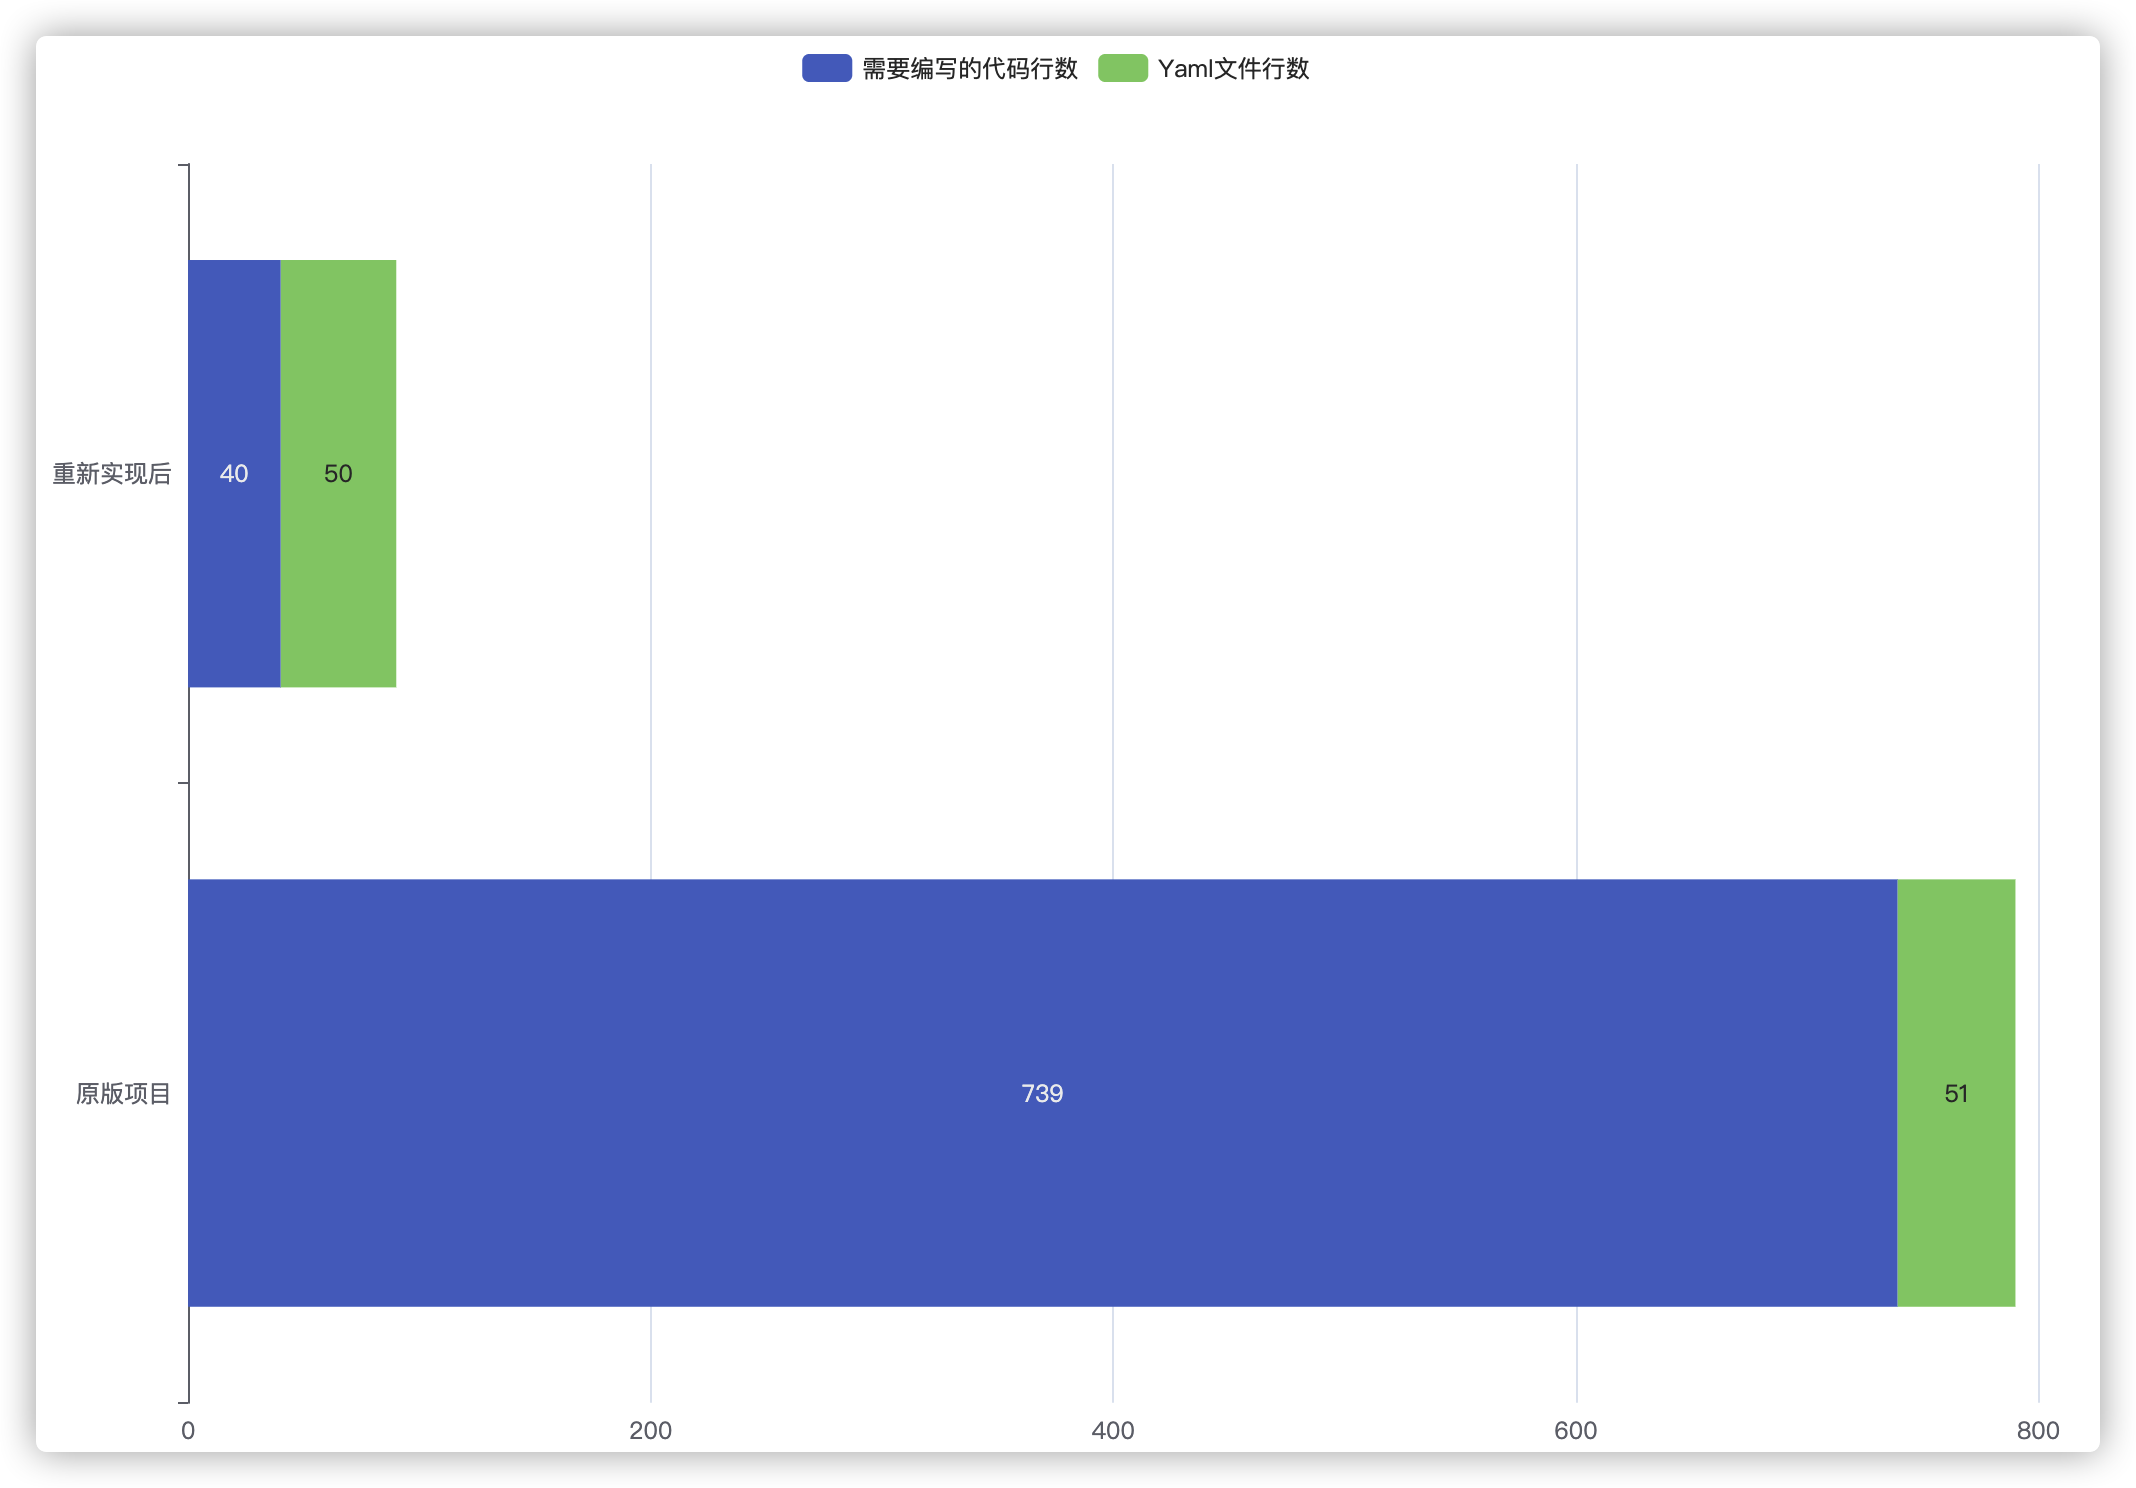
\includegraphics[width= 1\textwidth]{pics/sample-controller-cl.png}\\
  \caption{sample-controller原版与UC版代码行数比较}\label{fig:sample-controller-cl}
\end{figure}

\section{用例2:重新实现tf-operaotr}
\subsection{介绍}
tf-operator由kubeflow社区开发,项目地址为https://github.com/kubeflow/tf-operator,它提供了TFJob这个Kubernetes自定义资源,使其能够轻松地在Kubernetes上运行分布式或非分布式TensorFlow任务。
\subsection{实现}

\begin{lstlisting}[language=JavaScript,caption=tensorflowjob-controller的实现代码,label=listing:tensorflowjob-controller]
let tfjob = observed.parent;
let status = deepCopy(tfjob.status);
let observedPods = Object.values(observed.children['Pod.v1']);
let replicas = tfjob.spec.tfReplicaSpecs;
for (let rtype of Object.keys(replicas)) {
  let spec = replicas[rtype];
  let rt = rtype.toLowerCase();
  status.replicaStatuses[rtype] = {active: 0, succeeded: 0, failed: 0};
  let pods = filterPodsForReplicaType(observedPods, rt);
  let numReplicas = spec.replicas;
  let podSlices = getPodSlices(pods, numReplicas);
  for (let index = 0; index < podSlices.length; index++) {
    if (index < numReplicas) {
      desired.children.push(newSVC(tfjob, rtype, index));
    }
    let podSlice = podSlices[index];
    if (podSlice.length === 1) {
      let pod = podSLice[0];
      let exitCode = getContainerExitCode(pod);
      if (spec.restartPolicy === 'ExitCode') {
        if (pod.status.phase === 'Failed' && isRetryableExitCode(exitCode)) {
          updateJobConditions(status, 'Restarting', 'TFJobRestarting',
              `TFJob ${tfjob.metadata.name} is restarting because ${rtype} replica(s) failed.`);
          continue;
        }
      }
      if (pod.status.phase === 'Running') {
        status.replicaStatuses[rtype].active++;
      } else if (pod.status.phase === 'Succeeded') {
        status.replicaStatuses[rtype].succeeded++;
      } else if (pod.status.phase === 'Failed') {
        status.replicaStatuses[rtype].failed++;
      }
    }
    if (index < numReplicas) {
      let masterRole = isMasterRole(replicas, rtype, index);
      desired.children.push(newPod(tfjob, rt, index, spec, masterRole, replicas));
    }
  }
}
\end{lstlisting}

tf-operator依然用JavaScript实现,但实现逻辑相当复杂,总代码行数为408行,核心代码为代码段\ref{listing:tensorflowjob-controller}。原版tf-operator中的逻辑都转译了过来,包括根据不同的副本类型使用当前tfjob资源中相应的模版来创建Pod,为每一个Pod创建一个Service,分别统计每种副本的状态来更新tfjob的status等。

接下来借助kubeless将这个函数部署成web服务,部署命令为:

kubeless -n universalcontroller function deploy tensorflow-controller --runtime nodejs10 --from-file sync1.js --handler sync1.handler

之后在universalcontroller命名空间下会生成一个名叫tensorflow-controller的Service资源和一个名叫tensorflow-controller的Deployment资源,于是在集群内部就可以用http://tensorflow-controller.universalcontroller:8080访问这个服务,这个url就是要生成的controller使用的同步钩子。

\begin{lstlisting}[language=yaml,caption=tensorflowjob-controller的配置文件,label=listing:tensorflow-controller-config]
apiVersion: universalcontroller.njuics.cn/v1alpha1
kind: UniversalController
metadata:
  name: tensorflowjob-controller
spec:
  parentResource:
    apiVersion: mlhub.njuics.cn/v1alpha1
    resource: tensorflowjobs
  childResources:
    - apiVersion: v1
      resource: services
      updateStrategy:
        method: InPlace
    - apiVersion: v1
      resource: pods
      updateStrategy:
        method: ReCreate
  hooks:
    sync:
      webhook:
        url: "http://tensorflow-controller.universalcontroller:8080"
\end{lstlisting}

YAML文件\ref{listing:tensorflow-controller-config}是tensorflowjob-controller的声明式定义。

\subsection{对比总结}
原版tf-operator主要使用了client-go包,实现了一个标准的Operator,Go代码行数为17155,剔除使用代码生成工具生成的代码以及测试代码后代码行数为2344。在UniversalController之上实现的版本只需要四百多行JavaScript代码就能实现同样的功能。这个用例主要是为了展示UniversalController具备在实现复杂Operator时依然保持工作量相对较小的能力。图\ref{fig:tf-operator-cl}直观地展现了工作量的差距。

\begin{figure}[htbp]
  \centering
  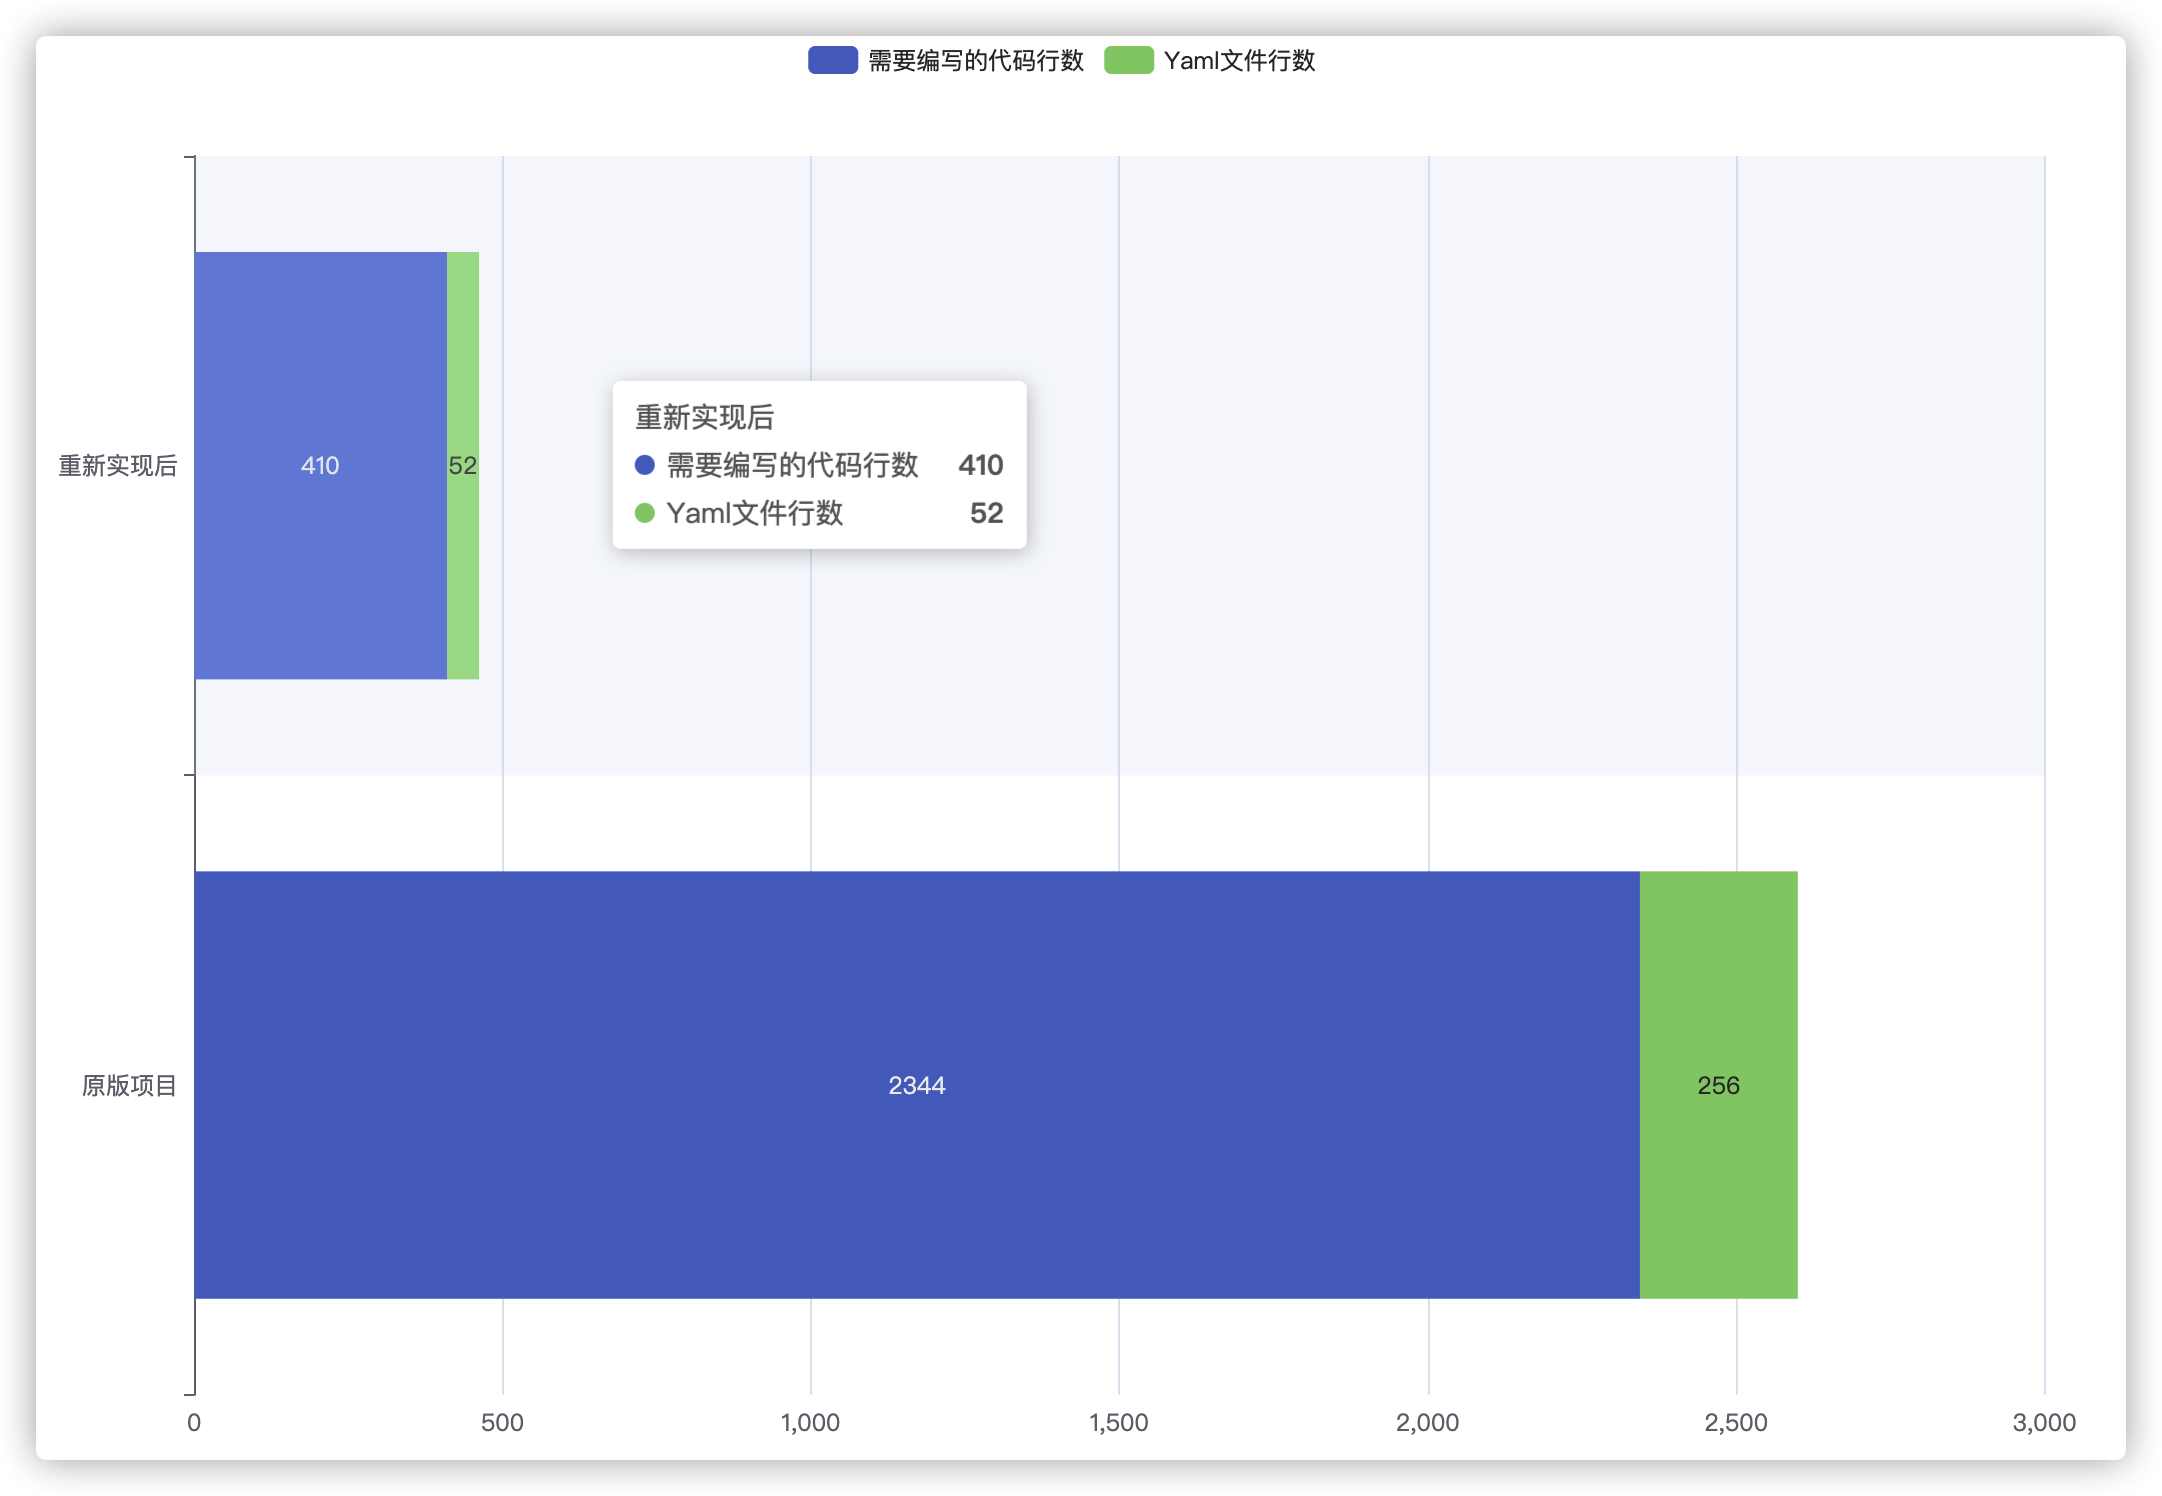
\includegraphics[width= 1\textwidth]{pics/tf-operator-cl.png}\\
  \caption{tf-operator原版与UC版代码行数比较}\label{fig:tf-operator-cl}
\end{figure}

\section{用例3:CatSet与滚动更新}
\subsection{介绍}
CatSet是对Kubernetes原生资源StatefulSet的重新实现,同时可以展示滚动更新的使用。
\subsection{实现}

\begin{lstlisting}[language=JavaScript,caption=生成Pod和PVC,label=listing:catset]
module.exports = {
  handler: (event, context) => {
    let observed = event.data;
    let desired = {status: {}, children: []};
    let catset = observed.parent;
    // Arrange observed Pods by ordinal.
    let observedPods = {};
    if (observed.children && observed.children['Pod.v1']) {
      for (let pod of Object.values(observed.children['Pod.v1'])) {
        let ordinal = getOrdinal(catset.metadata.name, pod.metadata.name);
        if (ordinal >= 0) observedPods[ordinal] = pod;
      }
    }
    if (observed.finalizing) {
      // If the parent is being deleted, scale down to zero replicas.
      catset.spec.replicas = 0;
      // Mark the finalizer as done if there are no more Pods.
      desired.finalized = (Object.keys(observedPods).length === 0);
    }
    for (var ready = 0; ready < catset.spec.replicas && isRunningAndReady(observedPods[ready]); ready++) ;
    desired.status = {replicas: Object.keys(observedPods).length, readyReplicas: ready};
    let desiredPods = {};
    for (let ordinal in observedPods) {
      desiredPods[ordinal] = newPod(catset, ordinal);
    }
    // Fill in one missing Pod if all lower ordinals are Ready.
    if (ready < catset.spec.replicas && !(ready in desiredPods)) {
      desiredPods[ready] = newPod(catset, ready);
    }
    // If all desired Pods are Ready, see if we need to scale down.
    if (ready === catset.spec.replicas) {
      let maxOrdinal = Math.max(...Object.keys(desiredPods));
      if (maxOrdinal >= catset.spec.replicas) {
        delete desiredPods[maxOrdinal];
      }
    }
    // List Pods in descending order, since that determines rolling update order.
    for (let ordinal of Object.keys(desiredPods).sort((a, b) => a - b).reverse()) {
      desired.children.push(desiredPods[ordinal]);
    }
    if (catset.spec.volumeClaimTemplates) {
      let desiredPVCs = {};
      for (let template of catset.spec.volumeClaimTemplates) {
        let baseName = `${template.metadata.name}-${catset.metadata.name}`;
        for (let i = 0; i < catset.spec.replicas; i++) {
          desiredPVCs[i] = newPVC(`${baseName}-${i}`, template);
        }
        // Also generate a desired state for existing PVCs outside the range.
        // PVCs are retained after scale down, but are deleted with the CatSet.
        if (observed.children && observed.children['PersistentVolumeClaim.v1']) {
          for (let pvc of Object.values(observed.children['PersistentVolumeClaim.v1'])) {
            if (pvc.metadata.name.startsWith(baseName)) {
              let ordinal = getOrdinal(baseName, pvc.metadata.name);
              if (ordinal >= catset.spec.replicas) desiredPVCs[ordinal] = newPVC(pvc.metadata.name, template);
            }
          }
        }
      }
      desired.children.push(...Object.values(desiredPVCs));
    }
    return desired;
  },
};
\end{lstlisting}

\begin{lstlisting}[language=yaml,caption=catset-controller的配置文件,label=listing:catset-controller-config]
---
apiVersion: universalcontroller.njuics.cn/v1alpha1
kind: UniversalController
metadata:
  name: catset-controller
spec:
  parentResource:
    apiVersion: mlhub.njuics.cn/v1alpha1
    resource: catsets
    revisionHistory:
      fieldPaths:
        - spec.template
  childResources:
    - apiVersion: v1
      resource: pods
      updateStrategy:
        method: RollingRecreate
        statusChecks:
          conditions:
            - type: Ready
              status: "True"
    - apiVersion: v1
      resource: persistentvolumeclaims
  hooks:
    sync:
      webhook:
        url: "http://catset-controller.universalcontroller:8080"
    finalize:
      webhook:
        url: "http://catset-controller.universalcontroller:8080"
\end{lstlisting}

\begin{lstlisting}[language=yaml,caption=CatSet资源示例,label=listing:catset-sample]
apiVersion: mlhub.njuics.cn/v1alpha1
kind: CatSet
metadata:
  name: nginx-backend
spec:
  serviceName: nginx-backend
  replicas: 3
  selector:
    matchLabels:
      app: nginx
  template:
    metadata:
      labels:
        app: nginx
        component: backend
    spec:
      terminationGracePeriodSeconds: 1
      containers:
      - name: nginx
        image: gcr.io/google_containers/nginx-slim:0.8
        ports:
        - containerPort: 80
          name: web
        volumeMounts:
        - name: www
          mountPath: /usr/share/nginx/html
  volumeClaimTemplates:
  - metadata:
      name: www
      labels:
        app: nginx
        component: backend
    spec:
      accessModes: [ "ReadWriteOnce" ]
      resources:
        requests:
          storage: 1Gi
\end{lstlisting}

YAML文件\ref{listing:catset-controller-config}是catset-controller的声明式定义。Yaml文件\ref{listing:catset-sample}是一个CatSet资源的示例,CatSet的spec结构与StatefulSet的spec结构完全一样。

CatSet的控制器依然用JavaScript实现,代码段\ref{listing:catset}是主逻辑,需要生成带编号的Pods和PVC(如果有的话),为了支持滚动更新,还要把Pods按照编号排好序再返回,因为滚动更新是按照调谐结果中子资源列表中的顺序逐个更新的。

\subsection{对比总结}
CatSet重新实现了StatefulSet,并且支持滚动更新。为了支持滚动更新,开发者只需要编写YAML文件\ref{listing:catset-controller-config}的第16到第21行,为pods子资源加上滚动更新策略,以及编写代码\ref{listing:catset}的第38行到第40行将期望存在的Pods按照序号降序排列即可。开发者总共只添加了9行代码就让CatSet支持了滚动更新,而为了让StatefulSet支持滚动更新,Kubernetes开发者改动了业务逻辑、模版文件、生成的代码,总共涉及到了超过9000行的改动\cite{statefulsetupdate}。UC提供的声明式接口帮助开发者快速地使自己的应用支持滚动更新。

%\section{用例4:Customize钩子的用法}
%\subsection{介绍}
%本文实现了globalconfigmap-operator,用于介绍Customize钩子的用法。
%\subsection{实现}
%
%\begin{lstlisting}[language=Python,caption=,label=listing:]
%
%\end{lstlisting}
%
%\begin{lstlisting}[language=yaml,caption=globalconfigmap-controller的配置,label=listing:globalconfigmap-controller-config]
%apiVersion: universalcontroller.njuics.cn/v1alpha1
%kind: UniversalController
%metadata:
%  name: globalconfigmap-controller
%spec:
%  generateSelector: true
%  parentResource:
%    apiVersion: mlhub.njuics.cn/v1alpha1
%    resource: globalconfigmaps
%  childResources:
%  - apiVersion: v1
%    resource: configmaps
%    updateStrategy:
%      method: InPlace
%  hooks:
%    sync:
%      webhook:
%        url: http://globalconfigmap-controller.universalcontroller/sync
%    customize:
%      webhook:
%        url: http://globalconfigmap-controller.universalcontroller/customize
%\end{lstlisting}
%
%yaml文件\ref{globalconfigmap-controller-config}是用于在UniversalController中注册一个控制器的配置文件。
%
%\subsection{总结}
%因为globalcomfigmap-operator需要把一个ConfigMap复制到每个命名空间,所以用户编写同步钩子时需要知道集群当前有哪些命名空间。

\section{性能测试}

Operator一般都不是计算型任务,运行时CPU的占用率极低,特别是在(超)小型集群中,接近于0。但是因为要监视资源,也就是订阅并且建立缓存,内存开销和网络开销呈线性增长。所以性能测试主要从这两个维度进行分析。

\subsection{实验环境}

在表\ref{table:test-env}所描述的集群上搭建了Kubernetes集群用于实验。
\begin{table}
  \centering
  \begin{tabular}{cp{60mm}c}
    \toprule
    \textbf{硬件类型} & \textbf{型号} & \textbf{规格} \\
    \midrule
    CPU  & Intel(R) Xeon(R) CPU E5-2630 v4 @ 2.20GHz  & 20核\\
    GPU  & NVIDIA 1080Ti   &  2 \\
    内存     & DDR4 & 128GB \\
    网卡    & Mellanox Technologies MT26448   & 10Gbps \\
    磁盘 & TOSHIBA MG04SCA20EN & 2TB \\
    \bottomrule
  \end{tabular}
  \caption{四节点集群的服务器配置}\label{table:test-env}
\end{table}

\subsection{对比方法}

我设计了六种场景,用于论证相比于部署多个Operators,使用UniversalController可以消耗更少的内存和网络带宽。每个场景准备前都要清理环境,重新安装Kubernetes,之后部署100个只执行“sleep 365d”的Pod当做负载。我还实现了一个donothing-operator,它的CRD为DoNothing,会订阅Pod和PVC,但是什么都不干。实现它的目的是为了与CatSet对比,CatSet也会订阅Pod和PVC。

接下来每个场景会安装不同的Operators:
\begin{itemize}
	\item \textbf{场景1}:不安装任何Operator。
	\item \textbf{场景2}:只安装UniversalController。
	\item \textbf{场景3}:只安装原版的tf-operator。
	\item \textbf{场景4}:先安装UniversalController,再安装重新实现的tf-operator。
	\item \textbf{场景5}:安装donothing-operator和原版的tf-operator。
	\item \textbf{场景6}:先安装UniversalController,再安装重新实现的tf-operator以及catset-operator。
\end{itemize}

一个Opeator在安装之后,首先会与api-server进行同步,建立它关心的资源的缓冲,所有启动之后会有一小段网络流量高峰,之后回落,再趋于平稳,内存也是先快速增长,之后趋于平稳。我会将每个场景中api-server在Operators启动后的前5分钟内上传的总数据量作为网络负载参考量,将之后5分钟内Operators所占用的总内存的平均值作为内存负载参考量。

\subsection{实验结果}
表\ref{table:test}汇总了各个场景的结果。场景1中没有任何Operator,但是每个节点的Kubelet都需要与api-server同步信息,所有也有很多数据需要传输。场景2中安装了UniversalController,但是UC它只会监听UC CRD,集群中没有任何UC CRD,所以api-server的网络负载几乎不变。场景3中tf-operator需要订阅TFJob、Pod、Service,所以api-server的网络负载增加了不少。

对比场景3和场景4可以看到,因为UC Controller自身带来的负载,重新实现的tf-operator的内存和网络负载都要比原版的tf-operator要高。

但是对比场景5和场景6可以看到,再增加一个operator后,场景5的内存和网络负载要更高,比场景3增长很多,而场景6与场景4的负载很接近。tf-operator和catset-operator都需要订阅Pod资源,但是当它们都部署在UniversalController之上时,Pod资源只会被订阅一次,这部分就不会带来额外的负载,catset-operator还需要订阅Service和CatSet,但是我们当前集群中主要的资源都是Pod,Service很少,还没有CatSet,所以也没有产生很多负载。

借助UniversalController的共享信息器(SharedInformer),当部署多个Operators时,部署在UniversalController之上要比每个单独部署占用更少的内存和网络带宽。
\begin{table}
  \centering
  \begin{tabular}{ccc}
    \toprule
    \textbf{场景编号} & \textbf{Operators内存总用量(MB)} & \textbf{5分钟内上传数据量(KB)} \\
    \midrule
    1  & 0 & 11995.14 \\
    2  & 12.52  &  12012.05 \\
    3  & 13.87  & 13297.24 \\
    4  & 19.18 &  13438.46 \\
    5  & 25.78  & 14529.64 \\
    6  & 21.93  & 13542.36 \\
    \bottomrule
  \end{tabular}
  \caption{性能测试}\label{table:test}
\end{table}

\section{小结}
本章设计了多个用例,用UniversalController实现了三个功能各异的Kubernetes Operators,验证了UniversalController可以简化Operator的实现,并且有很强的通用性。

本章设计的性能测试也证实UniversalController借助于共享通知者(sharedInformer),避免了重复订阅同一个资源,相比于一般的多控制器部署方式对内存和网络的占用更小。
%%%%%%%%%%%%%%%%%%%%%%%%%%%%%%%%%%%%%%%%%%%%%%%%%%%%%%%%%%%%%%%%%%%%%%%%%%%%%%%
% 学位论文的正文应以《结论》作为最后一章
\chapter{总结和展望}\label{chapter_concludes}
\section{工作总结}
随着云计算的蓬勃发展,新技术不断涌现。Docker和Kubernetes的出现更是重要的里程碑。Kubernetes已经成为了容器编排的实时标准,是云计算重要的基础设施。但是Kubernetes提供的现有APIs不一定能够很好的满足使用者的需求,使用者经常需要去扩展Kubernetes以更好的支持自己的应用的部署、更新和维护。最主流的Kubernetes扩展方式就是Kubernetes Operators,大量的Operators开始在开源社区出现。然而,编写一个Operator并不容易,具有相当高的门槛,并且需要付出大量的精力和时间。Operator开发人员需要一定程度的Kubernetes和分布式系统知识,需要写大量的模版代码或者使用代码生成工具,编写出的Operator帮助我们实现了应用程序的自动化运维,但是维护这个Operator却还是要给开发人员带来很大的负担。

本文提出了一种声明式的通用Kubernetes Operator,为用户开发Operator提供一种简单的新方式,让用户摆脱Go语言、Kubernetes开发工具包、代码生成工具的学习与使用成本,用更加声明式的方式开发Operator,将注意力完全集中在核心业务逻辑上,并且可以使用任意自己喜欢或熟悉的语言来实现一个标准优质的Operator。本文将该工具成为UniversalController,它自身也是一个Operator,底层实现是经典的控制器模式,但是把业务逻辑部分抽取出来托管给用户编写的hooks。

借助UniversalController提供的声明式API,用户在写核心业务逻辑时也可以获得平时使用yaml编写配置文件并使用kubectl apply部署相近的体验,只是需要改用json编写一些配置文件。如果用户已经很熟悉用kubectl apply去使用Kubernetes的声明式API来管理应用,那么就可以很容易地基于UniversalController实现一个Operator为应用的部署、更新、维护提供自动化流程而不必去学习Go语言或者如何使用Kubernetes客户端库,也不需要去学习使用代码生成工具。

\section{未来展望}
本文提出的工作将Kubernetes操作相关的代码从业务逻辑中提取了出来,用户不用再关注Kubernetes的Client API,让用户将开发工作集中在业务逻辑上,帮助用户减少了大量的开发工作。同时,本文仍然存在需要在未来工作中进行改进的地方。

本文提出的工作让用户将开发工作集中在业务逻辑上,但是用户必须借助serverless工具或者自己编写网络处理相关代码来启动一个web服务,以便与UniversalController对接。未来的工作中会加入更多的机制,例如gRPC或者嵌入式的脚本代码,让用户可以有更多的选择。或者可以将UniversalController的一部分封装成更加通用的库,提供一些方便的开发接口,开发者可以将业务逻辑实现成系统内部的代码调用,这样就不用将业务逻辑放在UniversalController的外部组件内,省去网络通信的开销。
%%%%%%%%%%%%%%%%%%%%%%%%%%%%%%%%%%%%%%%%%%%%%%%%%%%%%%%%%%%%%%%%%%%%%%%%%%%%%%%
% 致谢,应放在《结论》之后
%\begin{acknowledgement}
%  硕士漫漫三年这么快就过去了,在此期间我相识很多为我提供很多帮助或欢乐的人,由衷地感谢他们。
%首先,也是最主要感谢的是我的指导老师,曹春老师。在我的硕士阶段都及时适当的提点我,让我思路贯通,他的细心指导是我顺利完成研究的最大助力。
%我还要感谢我的朋友们,谢谢大家三年来给我的关心、信任和帮助,谢谢你们陪我走过人生一段美好时光。
%最后,深深感谢我的父母和亲人。这些年,您们无私而无微不至的关心和鼓 励,让我从不孤单。
%在此,我衷心感谢所有帮助我的人,没有你们我不可能完成这项工作,没有你们我的三年不会如此充实,真心感谢您们!
%\end{acknowledgement}

% 参考文献。应放在\backmatter之前。
% 推荐使用BibTeX,若不使用BibTeX时注释掉下面一句。
\nocite{*}
\bibliography{sample}
% 不使用 BibTeX
%\begin{thebibliography}{2}
%
%\bibitem{deng:01a}
%{邓建松,彭冉冉,陈长松}.
%\newblock {\em \LaTeXe{}科技排版指南}.
%\newblock 科学出版社,书号:7-03-009239-2/TP.1516, 北京, 2001.
%
%\bibitem{wang:00a}
%王磊.
%\newblock {\em \LaTeXe{}插图指南}.
%\newblock 2000.
%\end{thebibliography}

%%%%%%%%%%%%%%%%%%%%%%%%%%%%%%%%%%%%%%%%%%%%%%%%%%%%%%%%%%%%%%%%%%%%%%%%%%%%%%%
% 附录
%%%%%%%%%%%%%%%%%%%%%%%%%%%%%%%%%%%%%%%%%%%%%%%%%%%%%%%%%%%%%%%%%%%%%%%%%%%%%%%
% 书籍附件
\backmatter
%%%%%%%%%%%%%%%%%%%%%%%%%%%%%%%%%%%%%%%%%%%%%%%%%%%%%%%%%%%%%%%%%%%%%%%%%%%%%%%
% 作者简历与科研成果页,应放在backmatter之后
%\begin{resume}
%% 论文作者身份简介,一句话即可。
%\begin{authorinfo}
%\noindent 汪浩港,男,汉族,1996年12月出生,江苏省扬州人。
%\end{authorinfo}
%% 论文作者教育经历列表,按日期从近到远排列,不包括将要申请的学位。
%\begin{education}
%\item[2014年9月 --- 2018年6月] 中国矿业大学计算机科学与技术系 \hfill 本科
%\end{education}
%% 论文作者在攻读学位期间所发表的文章的列表,按发表日期从近到远排列。
%
%% 论文作者在攻读学位期间参与的科研课题的列表,按照日期从近到远排列。
%\begin{projects}
%	\item 国家重点研发项目:软件定义的人机物融合云计算支撑技术与平台(2018YFB004805),2018年5月-2021年4月
%\end{projects}
%\end{resume}

%%%%%%%%%%%%%%%%%%%%%%%%%%%%%%%%%%%%%%%%%%%%%%%%%%%%%%%%%%%%%%%%%%%%%%%%%%%%%%%
% 生成《学位论文出版授权书》页面,应放在最后一页
\makelicense

%%%%%%%%%%%%%%%%%%%%%%%%%%%%%%%%%%%%%%%%%%%%%%%%%%%%%%%%%%%%%%%%%%%%%%%%%%%%%%%
\end{document}
